\documentclass{ut-thesis-custom}

% ============================================================
% METADATA (ut-thesis preamble commands)
% ============================================================
\author{Sebastien Psarianos}
\title{A 2D Ionospheric Shell Model as a Boundary Condition
       for a Global MHD Space Weather Simulation}
\degree{Bachelor of Science}
\department{Physics}
\gradyear{\the\year}

% ============================================================
% PACKAGES
% ============================================================
\usepackage{amsmath}
\usepackage{amssymb}
\usepackage{graphicx}
\usepackage{booktabs}
\usepackage[numbers]{natbib}
\usepackage[colorlinks=true,
            linkcolor=black,
            citecolor=black,
            urlcolor=blue,
            pdftitle={A 2D Ionospheric Shell Model as a Boundary Condition
                      for a Global MHD Space Weather Simulation},
            pdfauthor={Sebastien Psarianos}]{hyperref}
\usepackage{cleveref}
\usepackage{caption}
\usepackage{subcaption}
\usepackage{float}
\usepackage{physics}
\usepackage{listings}
\usepackage{xcolor}
\usepackage{tikz}
\usepackage{standalone}
\usepackage{bm}
\usetikzlibrary{positioning, arrows.meta, fit, backgrounds, calc}
\usepackage{parskip}

% ============================================================
% COLORS
% ============================================================
\definecolor{capfill}{RGB}{200,225,240}
\definecolor{capedge}{RGB}{70,130,180}
\definecolor{polecol}{RGB}{204,51,51}
\definecolor{adjcol}{RGB}{230,120,50}
\definecolor{gridcol}{RGB}{50,50,80}
\definecolor{ringcol}{RGB}{140,140,160}
\definecolor{loncol}{RGB}{170,170,190}
\definecolor{annotcol}{RGB}{80,80,80}
\definecolor{stencilA}{RGB}{0,150,130}
\definecolor{stencilB}{RGB}{130,50,180}

% ============================================================
% CUSTOM COMMANDS
% ============================================================
\newcommand{\sigp}{\Sigma_P}
\newcommand{\sigh}{\Sigma_H}
\newcommand{\sigz}{\Sigma_0}

\newcommand{\jR}{j_R}
\newcommand{\RE}{R_E}

\newcommand{\C}{\mathcal{C}}
\newcommand{\parC}{\partial\mathcal{C}}

\newcommand{\placeholder}[2][0.9]{%
	\begin{center}
		\fcolorbox{black}{gray!20}{%
			\parbox{#1\textwidth}{%
				\centering\vspace{1.5cm}
				\textit{#2}
				\vspace{1.5cm}
			}%
		}
	\end{center}
}


\setcounter{tocdepth}{2}
\begin{document}
\frontmatter
\maketitle
\begin{abstract}

	Accurate modeling of space weather is integral to the security of infrastructure both on the ground and in orbit. Historic damage caused by geomagnetic storms has been assessed as likely avoidable with modern operational space weather modeling~\cite{economic_eastwood_2017}, of which accurate modeling of the magnetosphere-ionosphere coupled system is a key component. Ionospheric modeling relies on empirical values for the ionospheric conductivity that continue to evolve~\citep{cousins2015, moen1993, hardy1987}. This thesis establishes an expandable framework for magnetohydrodynamics coupling problems that is built with interchangeable physical models in mind to account for the evolving landscape of empirical models. The model described in this thesis is a 2D spherical-shell ionosphere model solving the~\citet{goodman1995} ionospheric surface equation with the~\citet{amm1996} conductivity tensor. The ionosphere code presented provides empirical conductivity models for the auroral and extreme ultraviolet-driven conductivities in a modular framework supporting expansion. The ionospheric surface equation is discretized, with a divergence theorem boundary condition that preserves pole continuity as a built-in constraint. The solve time of the model was improved from approximately 140 to 10 seconds on a $512\times256$ grid, achieved with a MueLu-preconditioned GMRES solver optimized using a parameter sweep study. Model output shows behaviour consistent with the two-cell pattern of ionosphere potentials for a southward IMF~\cite{kelley2009}. This model provides a framework for MHD coupling problems that is agnostic to the individual physical models it comprises.
\end{abstract}

\begin{acknowledgements}
	I would like to thank Dr. Groth for the opportunity to contribute to this project. I am grateful for the guidance he provided as I learned more about this field, and the help working through the harder problems.
\end{acknowledgements}

\tableofcontents
\listoffigures
\listoftables

% ------------------------------------------------------------
% MAIN MATTER
% ------------------------------------------------------------
\mainmatter

\chapter{Introduction}
\label{chap:introduction}
Accurate space weather modelling is essential to protecting critical technological infrastructure on Earth and in orbit. In March 1989, the largest geomagnetic storm of the space age, caused by two coronal mass ejections, initiated a widespread power outage in the Hydro-Quebec power grid \citep{21st_boteler_2019}. Estimates for the economic cost of such a blackout range from billions of dollars to trillions on the extreme end~\citep{economic_eastwood_2017}. Historical events such as a 2003 blackout in Sweden have been assessed as being likely avoidable with modern operational space weather modeling~\citep{economic_eastwood_2017}, showing the value of continued advancement in modeling accuracy.

Ionospheric current systems, driven by the magnetosphere, can induce rapidly varying magnetic fields on the surface of the Earth that in turn drive geomagnetically induced currents (GICs)~\citep{scientific_eastwood_2017}. These GICs can cause blackouts and destroy infrastructure on the ground. Therefore, modeling of the magnetosphere-ionosphere coupling is a key piece in mitigating the effects of geomagnetic activity.

The Earth's magnetosphere is strongly coupled to the ionosphere, which closes the field-aligned currents in the magnetosphere. The ionosphere acts like a load in the global magnetospheric circuit, dissipating the energy produced by field-aligned currents originating in the magnetosphere~\citep{impacts_liu_2023}. The modeling of the magnetospheric system is largely dependent on empirical models for the ionospheric conductivity that are frequently updated to improve accuracy~\citep{moen1993, goodman1995, cousins2015}. This thesis presents an ionosphere model built with modularity and extensibility as a design factor, allowing for space weather forecasting across a wide-selection of physical models.

The remainder of the thesis is organized as follows. Chapter 2 describes the empirical and physical models used to compute ionospheric conductivity. Chapter 3 shows the numerical implementation of the~\citet{goodman1995} ionosphere shell approximation, and expands on problematic polar behaviour and solver performance. Chapter 4 presents resulting potential distributions from the model with a southward IMF produced by the magnetosphere model described in~\citet{global_groth_2000}. Chapter 5 concludes with the future extensions planned for this application and further optimizations.

\section{Height Integrated Conductivities}
\label{sec:height_integrated_conductivities}
To understand the role that the Earth plays in completing the magnetosphere's field-aligned currents, it is important to accurately understand how the conductivity of the ionosphere dissipates the energy generated in the magnetosphere. Ohm's law is used in~\citet{goodman1995} to derive the equation used to complete the field-aligned currents and the conductivity tensor $\bm\sigma$ acts as the dissipative term that provides the load.
\begin{equation}
	\bm j = \bm\sigma\cdot \nabla\psi
	\label{eq:ohms_law}
\end{equation}
For ionospheric physics, the conductivity tensor is primarily represented as consisting of the Hall, Pedersen and parallel conductivities. These conductivities can be defined using the following tensor representation where $\bm B$ is taken to be parallel to the $z$-axis~\citep{kelley2009}:
\begin{equation*}
	\bm\sigma = \begin{pmatrix}
		\sigma_P & -\sigma_H & 0        \\
		\sigma_H & \sigma_P  & 0        \\
		0        & 0         & \sigma_0
	\end{pmatrix}
\end{equation*}
These conductivities can also be derived from physical plasma parameters, as shown in this example from~\citep{kelley2009}.
\begin{equation}
	\begin{aligned}
		\sigma_{P} & =ne\left[\frac{b_i}{1+\kappa_i^2}+\frac{b_e}{1+\kappa_e^2}\right]                    \\
		\sigma_{H} & =(ne/B) \left[\frac{\kappa_e^2}{1+\kappa_e^2}+\frac{\kappa_i^2}{1+\kappa_i^2}\right] \\
		\sigma_{0} & = ne(b_i-b_e)
		\label{eq:physical_conduct}
	\end{aligned}
\end{equation}
Where $n$ is the plasma number density, $e$ is the elementary charge, $B$ is the magnetic field magnitude, $b_i, b_e$ are the ion and electron mobilities and $\kappa_i,\kappa_e$ are the magnetization parameters. This shows a linear relationship between the density of charged particles in the ionosphere and its associated conductivity.

The height integrated conductivities are calculated by integrating the conductivity of each of these terms through the height of the ionosphere as follows~\citep{goodman1995}:
\begin{equation*}
	\Sigma_i = \int_{r_1}^{r_2} \bm\sigma \dd{R}
\end{equation*}
These height integrated conductivities are used in the ionospheric surface equation that is described in the next section. In order to use these conductivities on a spherical coordinate system, the Hall, Pedersen and parallel bases must be converted to be used in a spherical coordinate system. Since the direction these conductances correspond to is dependent on the magnetic field direction, \citet{amm1996} uses a dipole approximation of the Earth's magnetic field to describe the following tensor:
\begin{equation}
	\Sigma_{Amm} = \begin{pmatrix}
		0 & 0                      & 0                   \\
		0 & \Sigma_{\theta \theta} & \Sigma_{\theta\phi} \\
		0 & \Sigma_{\phi \theta}   & \Sigma_{\phi\phi}   \\
	\end{pmatrix} =
	\begin{pmatrix}
		0 & 0                                          & 0                                                \\
		0 & \frac{\Sigma_0\Sigma_P}{C}                 & \frac{\Sigma_0\Sigma_H (-\cos\varepsilon)}{C}    \\
		0 & \frac{\Sigma_0\Sigma_H \cos\varepsilon}{C} & \Sigma_P + \frac{\Sigma_H^2\sin^2\varepsilon}{C} \\
	\end{pmatrix}
	\label{eq:conductivity_tensor}
\end{equation}
This provides a conductivity tensor that allows for computation to be performed in spherical coordinates. Here $C$ and $\sin\varepsilon, \cos\varepsilon$ are defined:
\begin{align*}
	C                = \Sigma_0\cos^2\varepsilon + \Sigma_P \sin^2\varepsilon \\
	\cos\varepsilon  = - \frac{2\cos\theta}{\sqrt{1+3\cos^2\theta}}           \\
	\sin\varepsilon  =  \frac{\sin\theta}{\sqrt{1+3\cos^2\theta}}
\end{align*}
The Hall and Pedersen conductivities are readily available through empirical models. The practical implementation of the conductivity in the simulation is described in detail in Chapter~\ref{chap:conductivity}.
\section{The Ionosphere Surface Equation}
This ionospheric model provides a boundary condition for a global magnetospheric MHD model through a 2D shell representing the magnetosphere-ionosphere boundary.~\citet{goodman1995} derives an expression for the potential on the surface of the magnetosphere-ionosphere boundary layer using a combination of the radial current divergence and Ohm's law (Equation~\ref{eq:ohms_law}) that is displayed here:
\begin{equation}
	\nabla \cdot \bm j = \frac1{R^2}\pdv{R^2j_R}{R} + \nabla_\perp \cdot(\bm\sigma\cdot \nabla\psi)_\perp
	\label{eq:radcurr_divergence}
\end{equation}
By integrating Equation~\ref{eq:radcurr_divergence} through an altitude range $r_1 < R < r_2$ representative of the ionosphere region, Goodman arrives at the following expression for the ionospheric current system on the magnetosphere-ionosphere boundary.
\begin{equation}
	j_R(R_E) = \left[\nabla_\perp \cdot (\Sigma \cdot \nabla\psi)_\perp\right]
	\label{eqn:continuity_eqn}
\end{equation}
Where $R_E$ is the radius of the Earth; $j_R$ is the component of the current density that is radial to the surface of the ionosphere; $\Sigma$ is the height integrated conductivity tensor described in Section~\ref{sec:height_integrated_conductivities} and $\psi$ is the potential along the ionosphere. Here simplifying assumptions are made, see~\citep{goodman1995} for the full derivation. Equation~\ref{eqn:continuity_eqn} provides an expression that relates the field-aligned currents as a source term to the ionospheric potential. This equation is used to model the interactions of the field-aligned currents with the ionospheric region.
\section{Design Philosophy}
Because strategies for modeling the various components of the ionosphere continue to evolve, the structure of this application was designed to remain agnostic to implementation details of any individual component. The application is built from the ground up with configurability and extensibility in mind. This is achieved primarily through the interfaces defined for various portions of the application such as boundary conditions, governing equations and conductivity models. These interfaces allow new models to be easily integrated into the system by simply implementing a common interface. Figure~\ref{diag:full_flow2} displays the structure of the application, showing these distinct sections of the application, interfacing through common interface layers.
\begin{figure}[H]
	\centering
	\includestandalone[width=\textwidth]{diagrams/ApplicationFLow}
	\caption{Application structure diagram displaying the data flow of the solver and conductivity model structure. Displays the distinct regions of the application and the global configuration provided by the YAML configuration.}
	\label{diag:full_flow2}
\end{figure}

The application makes use of a YAML configuration throughout the application, allowing the application to be reconfigured on the fly. This opens up the possibility of cross-testing of different conductivity models, equations and simulation parameters without recompilation. A more comprehensive breakdown of the conductivity and solver portions of the application are given in Chapters~\ref{chap:conductivity} and~\ref{chap:implementation} respectively. The numerical backbone of the system is the Trilinos~\citep{TrilinosPaper} scientific computing framework along with the Tpetra~\citep{TpetraPaper} package. These packages provide the solvers and linear algebra utilities that are used throughout the simulation and provide the MPI utilities that allow for problem parallelization.


\chapter{Conductivity Modelling}
\label{chap:conductivity}
The conductivity of the ionosphere is the primary factor in the ionospheric continuity equation coefficients as proposed by~\citet{goodman1995} (Equation~\ref{eqn:continuity_eqn}). As discussed in Section~\ref{sec:height_integrated_conductivities}, the charged particle density is a driving factor in the variation of height integrated conductivities. The variation in the levels of charged particles in the ionosphere occurs due to both incident extreme ultraviolet (EUV) rays from the sun causing ionization in the ionosphere and auroral precipitation along the magnetic field lines~\citep{cousins2015}. Both of these are available through multiple empirical models, see \citet{moen1993,cousins2015, hardy1987}. This application has been designed to be agnostic to the choice of conductivity model to allow new models to be added and swapped without recompilation. In this section the conductance models that are currently implemented will be discussed along with plans for future conductivity model support, and the structure of this model's conductivity modeling.
\section{EUV Conductivities}
\label{sec:euv_conductivity}
The first main source of conductivity within the ionosphere is the ionization of particles in the ionosphere due to incident extreme ultraviolet radiation. This is the primary contribution to conductivity in the low latitude regions of the Earth. Even at high latitudes, when the auroral contribution is low the Hall and Pedersen conductivities are primarily driven by variations in solar EUV radiation~\citep{moen1993}.
\subsection{Moen Brekke EUV Conductivity Model}
The EUV conductivity model that has been implemented currently is the empirical model produced by \citet{moen1993}. This model provides an empirical formula for the EUV driven Hall and Pedersen conductivity as a function of F10.7 solar flux level $S_a$ and solar zenith angle $\chi$. This data is produced from EISCAT incoherent scatter data of the electron density profiles.
\begin{equation}
	\Sigma_H(\chi, S_a) = S_a^{0.53}(0.81\cos\chi + 0.54\cos^{1/2}\chi)
\end{equation}
\begin{equation}
	\Sigma_P(\chi, S_a) = S_a^{0.49}(0.34\cos\chi + 0.93\cos^{1/2}\chi)
\end{equation}
Figure~\ref{fig:euvPedersonVsSeason} displays EUV conductivity contributions to the height integrated Pedersen conductivity over three different dates. Seasonal variation can result in different distributions of conductivity through the ionosphere. This can have large effects on the final solution to Equation~\ref{eqn:continuity_eqn} as this can greatly influence behaviour on the poles. This is explored further in Chapter~\ref{chap:results}. This seasonal variation is provided by differing solar zenith angle distributions at different times of the year. The process of calculating the solar zenith angle is discussed in Section~\ref{sec:conductivity_implementation}, and the F10.7 solar flux levels are configurable through the YAML application configuration file.
\begin{figure}[H]
	\centering
	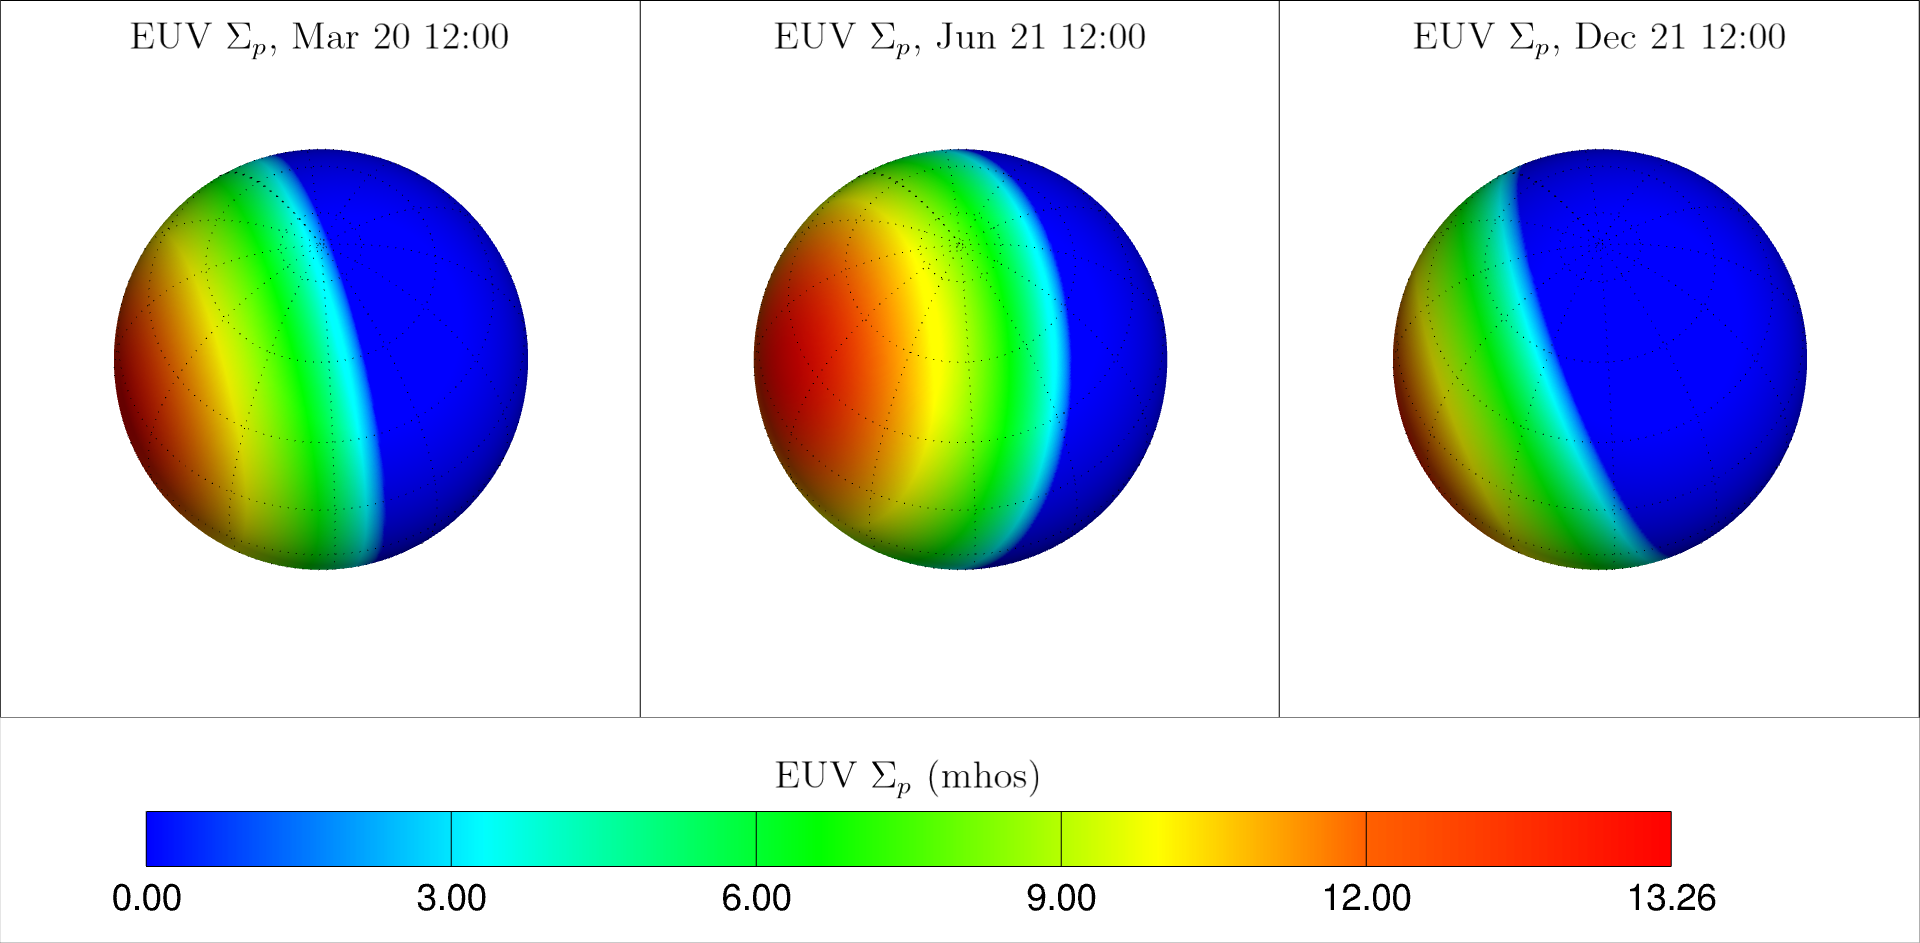
\includegraphics[width=\textwidth]{figures/euvlPedersonVsSeason.png}
	\caption{EUV-driven Pedersen conductance $\Sigma_p$ (mhos) for equinox (Mar 20), summer (Jun 21), and winter (Dec 21) at 12:00 UT, showing the seasonal variation of EUV conductivity.}
	\label{fig:euvPedersonVsSeason}
\end{figure}
\section{Auroral Conductivities}
The second main source of the ionospheric conductivity is through electrons introduced to the ionosphere through auroral precipitation. The strong magnetosphere-ionosphere coupling along field lines drives particle precipitation. Electrons precipitate into the ionosphere along magnetic field lines~\citep{hardy1987}, increasing the conductivity levels as discussed in Section~\ref{sec:height_integrated_conductivities}. Due to the structure of the Earth's magnetic field, this precipitation primarily occurs at high latitudes~\citep{hardy1987}. Considering that the high latitude region acts as the primary interface for magnetosphere-ionosphere coupling, the accuracy of the conductivities in this region is of utmost importance to the accuracy of the model~\citep{hardy1987}.

\subsection{Hardy Conductivity Model}
The auroral conductivity model that is currently implemented is the empirical model produced by \citet{hardy1987}. This paper used particle flux measurements from the SSJ/3 detectors aboard the DMSP F2 and F4 satellites and the CRL-251 detector aboard P78-1 to model the global auroral precipitation, following the conductivity derivation approach of~\citet{spiro1982}. The Hardy model models the auroral Hall and Pedersen conductivities using the Epstein transition function (Equation~\ref{eq:epstein_transition}).
\begin{equation}
	e(h) = r + S_1(h - h_0) + (S_2 - S_1) \cdot \ln\left\{
	\frac{1 - S_1/(S_2 e^{-(h-h_0)})}{1 - (S_1/S_2)}\right\}
	\label{eq:epstein_transition}
\end{equation}
The four values in this function are provided by the paper as sixth order Fourier series coefficients. These coefficients are binned by the magnetic activity index $K_p$ and the coefficients are then computed using a Fourier series with magnetic local time as the parameter as shown in Equation~\ref{eq:fourier_series}. These Fourier series provide the peak latitude ($h_0$), and the amplitude and slope parameters ($r$, $S_1$, $S_2$). The magnetic latitude is determined by the corresponding position on the grid.
\begin{equation}
	a(T) = \sum_{n=0}^{6}\left\{C_n^a \cos\left[\frac{n\pi T}{12}\right]
	+ S_n^a \sin\left[\frac{n\pi T}{12}\right]\right\}
	\label{eq:fourier_series}
\end{equation}
This provides a function for the Hall and Pedersen conductivities that is a function of the magnetic local time, magnetic activity index and magnetic latitude. The calculation of the magnetic local time required additional models to be implemented within the application. The magnetic activity index ($K_p$) is configurable through the YAML configuration file. The calculation of magnetic local time and the application structure is discussed further in Section~\ref{sec:conductivity_implementation}.

\begin{figure}[H]
	\centering
	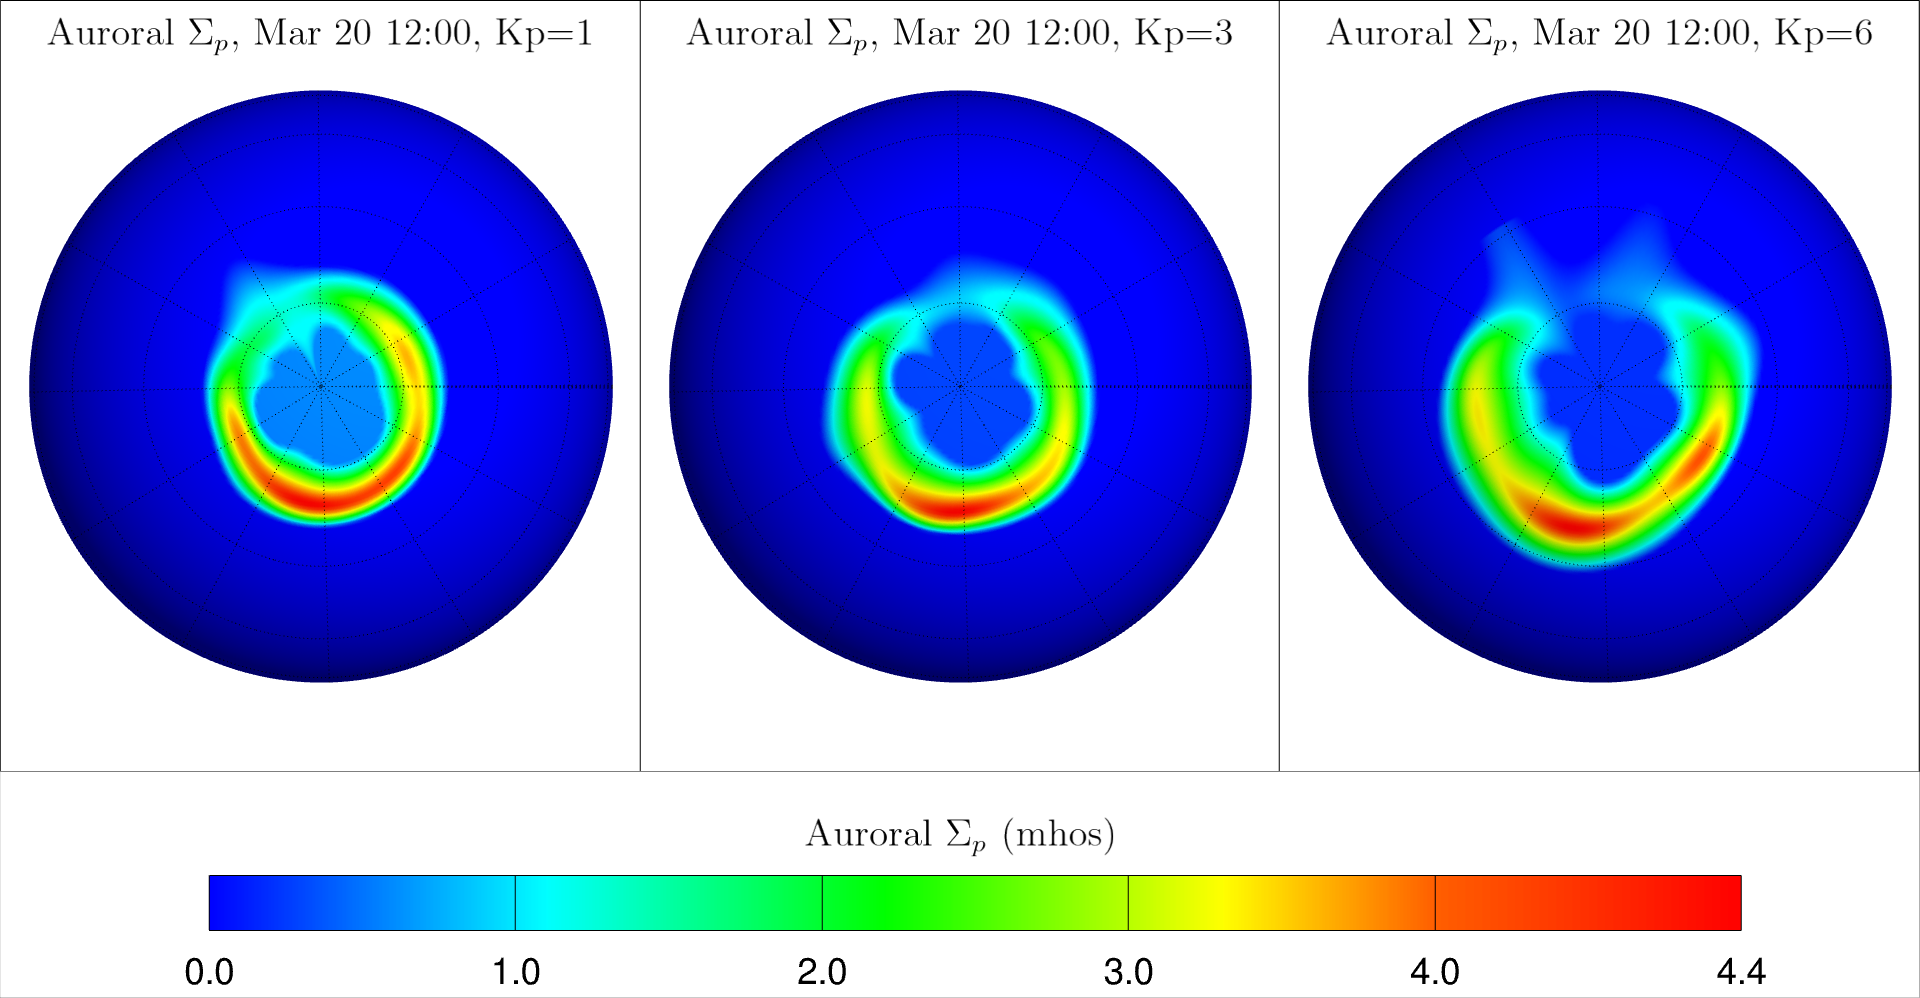
\includegraphics[width=\textwidth]{figures/auroralPedersonVsKp.png}
	\caption{Auroral Pedersen conductance $\Sigma_p$ (mhos) for $K_p = 1$, $3$, and $6$ on (Mar 20, 12:00), showing the expansion of the auroral conductance with increasing geomagnetic activity.}
	\label{fig:auroralPedersonVsKp}
\end{figure}
Figure~\ref{fig:auroralPedersonVsKp} displays three sample conductivity distributions for the height integrated Pedersen conductivity from the Hardy model over three different geomagnetic activity levels. The expansion of the auroral oval at high $K_p$ values can be seen clearly.

\section{Conductivity Combination}
To combine the two sources of conductivity, \citet{wallis1981} describes an approximation for determining the total conductivity from the auroral and EUV conductivities. This involves taking the root mean squared summation of the two conductivities as shown in Equation~\ref{eq:cond_combination}.
\begin{equation}
	\Sigma_{i, total} = \sqrt{\Sigma_{i, auroral}^2 + \Sigma_{i, EUV}^2}
	\label{eq:cond_combination}
\end{equation}
This was the method that was chosen for combining the contributions from each of the conductivity models. \citet{wallis1981} found the error of this approach to be $\sim$ 15\% and $\sim$ 7\% for $\Sigma_H$ and $\Sigma_P$ respectively when $\Sigma_{i,auroral} \approx \Sigma_{i,EUV}$. Therefore, this is not a good approximation for regions where both the auroral and EUV conductivities are contributing similarly. Due to the differing latitudes between the peak EUV-driven conductivity and the auroral conductivity, this error will by mainly focused on a band of mid-latitude points where the values are similar. Figure~\ref{fig:totalConductivity} shows the total conductivity computed within the simulation both with auroral and EUV contributions for both the Hall and Pedersen conductances. This is an example case of a low error combination due to the distributions of the EUV contribution and the auroral contribution being relatively distinct.
\begin{figure}[H]
	\centering
	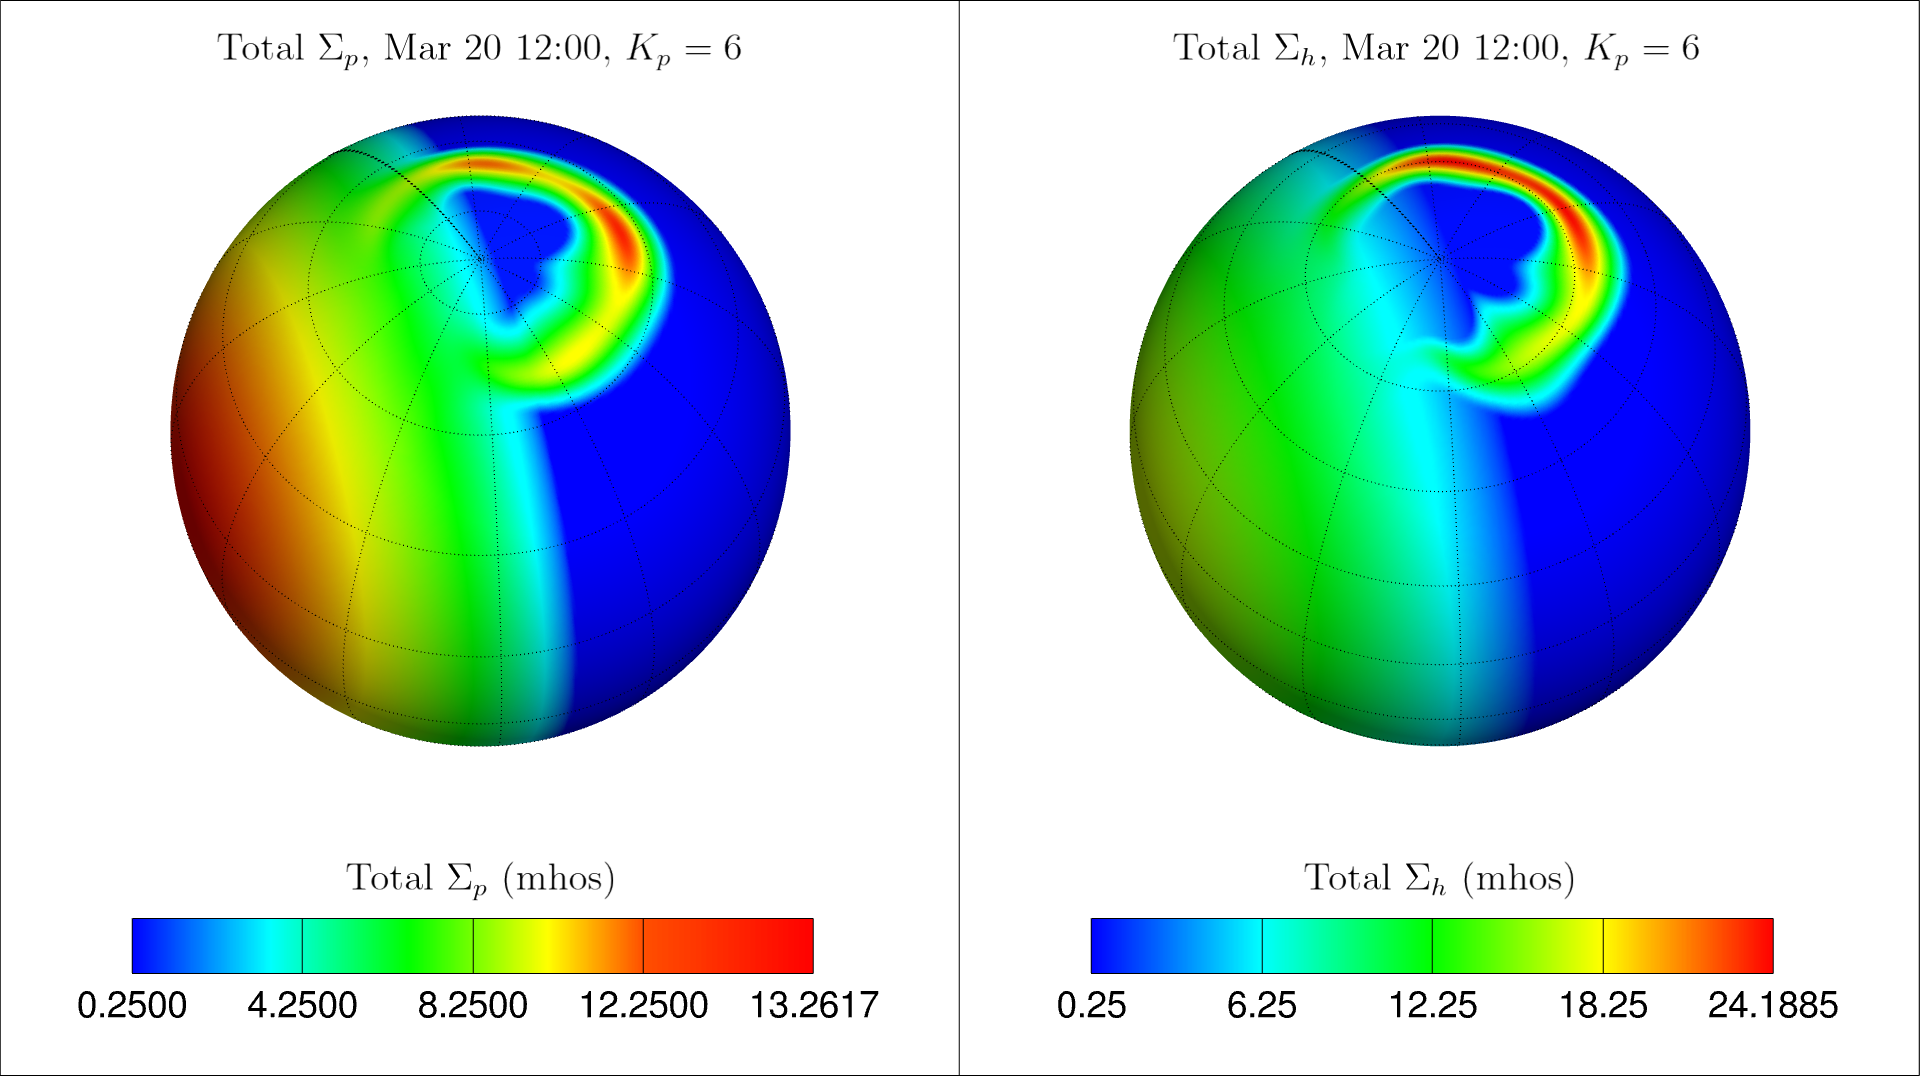
\includegraphics[width=\textwidth]{figures/totalConductivity.png}
	\caption{Total Pedersen ($\Sigma_p$) and Hall ($\Sigma_h$) conductances (mhos) for $K_p = 6$ at equinox (Mar 20, 12:00), combining EUV and auroral contributions.}
	\label{fig:totalConductivity}
\end{figure}

\section{Implementation}
\label{sec:conductivity_implementation}
To facilitate extensibility, the application was designed to be as configurable as possible without recompilation. Even though only one model is implemented so far within this system, the conductivity models implement an abstract interface and are injected through a factory function. This allows for the ability to hot-swap the conductivity models without recompilation when new ones are added. Additionally, new conductivity models can be built in the application by implementing the existing interface. Figure~\ref{diag:conductivity_diagram} shows the structure of the conductivity models that are currently implemented.
\begin{figure}[H]
	\centering
	\includestandalone[width=0.7\textwidth]{diagrams/ConductivityDiagram}
	\caption{Data flow diagram showing the structure of the conductivity model. Conductance tensor at the bottom is fed into the solver portion of the application through an abstract interface. The full system diagram is available in Figure~\ref{diag:full_flow2}.}
	\label{diag:conductivity_diagram}
\end{figure}
The auroral and EUV conductivity models required computation of the magnetic local time and solar zenith angle respectively. To achieve this, some additional small models were included in the application as seen in Figure~\ref{diag:conductivity_diagram}. These provided the ability to convert between magnetic dipole coordinates and geographic coordinates and to compute the solar zenith angle and magnetic local time.

The solar zenith angle is determined for all points on the grid using the third method described in~\citet{grena2012}. This provides the ability to compute the solar zenith angle for all points on the globe from a date and time configurable within a YAML configuration file. The solar zenith angle model required geographical coordinates, while the main coordinate system used in the ionosphere model is magnetic dipole coordinates. To make this conversion, the geographic to dipole conversion matrix described in~\citet{laundal2017} was included to create a rotational matrix that allowed for conversion between the two coordinate systems. By using the latest IGRF magnetic field coefficients available in \citet{igrf2024}, the dipole rotational matrix was then constructed. This matrix was used for coordinate transformations when required. The dipole matrix is interpolated between five year epochs using the provided parameters in~\citep{igrf2024}.

Figure~\ref{fig:mltAlignment} displays the magnetic local time as calculated in the ionosphere model. The magnetic local time is calculated by solving for the subsolar point (the point at which the sun's incidence is perpendicular to the Earth) and using that to calculate the relative times for all points on the grid.
\begin{figure}[H]
	\centering
	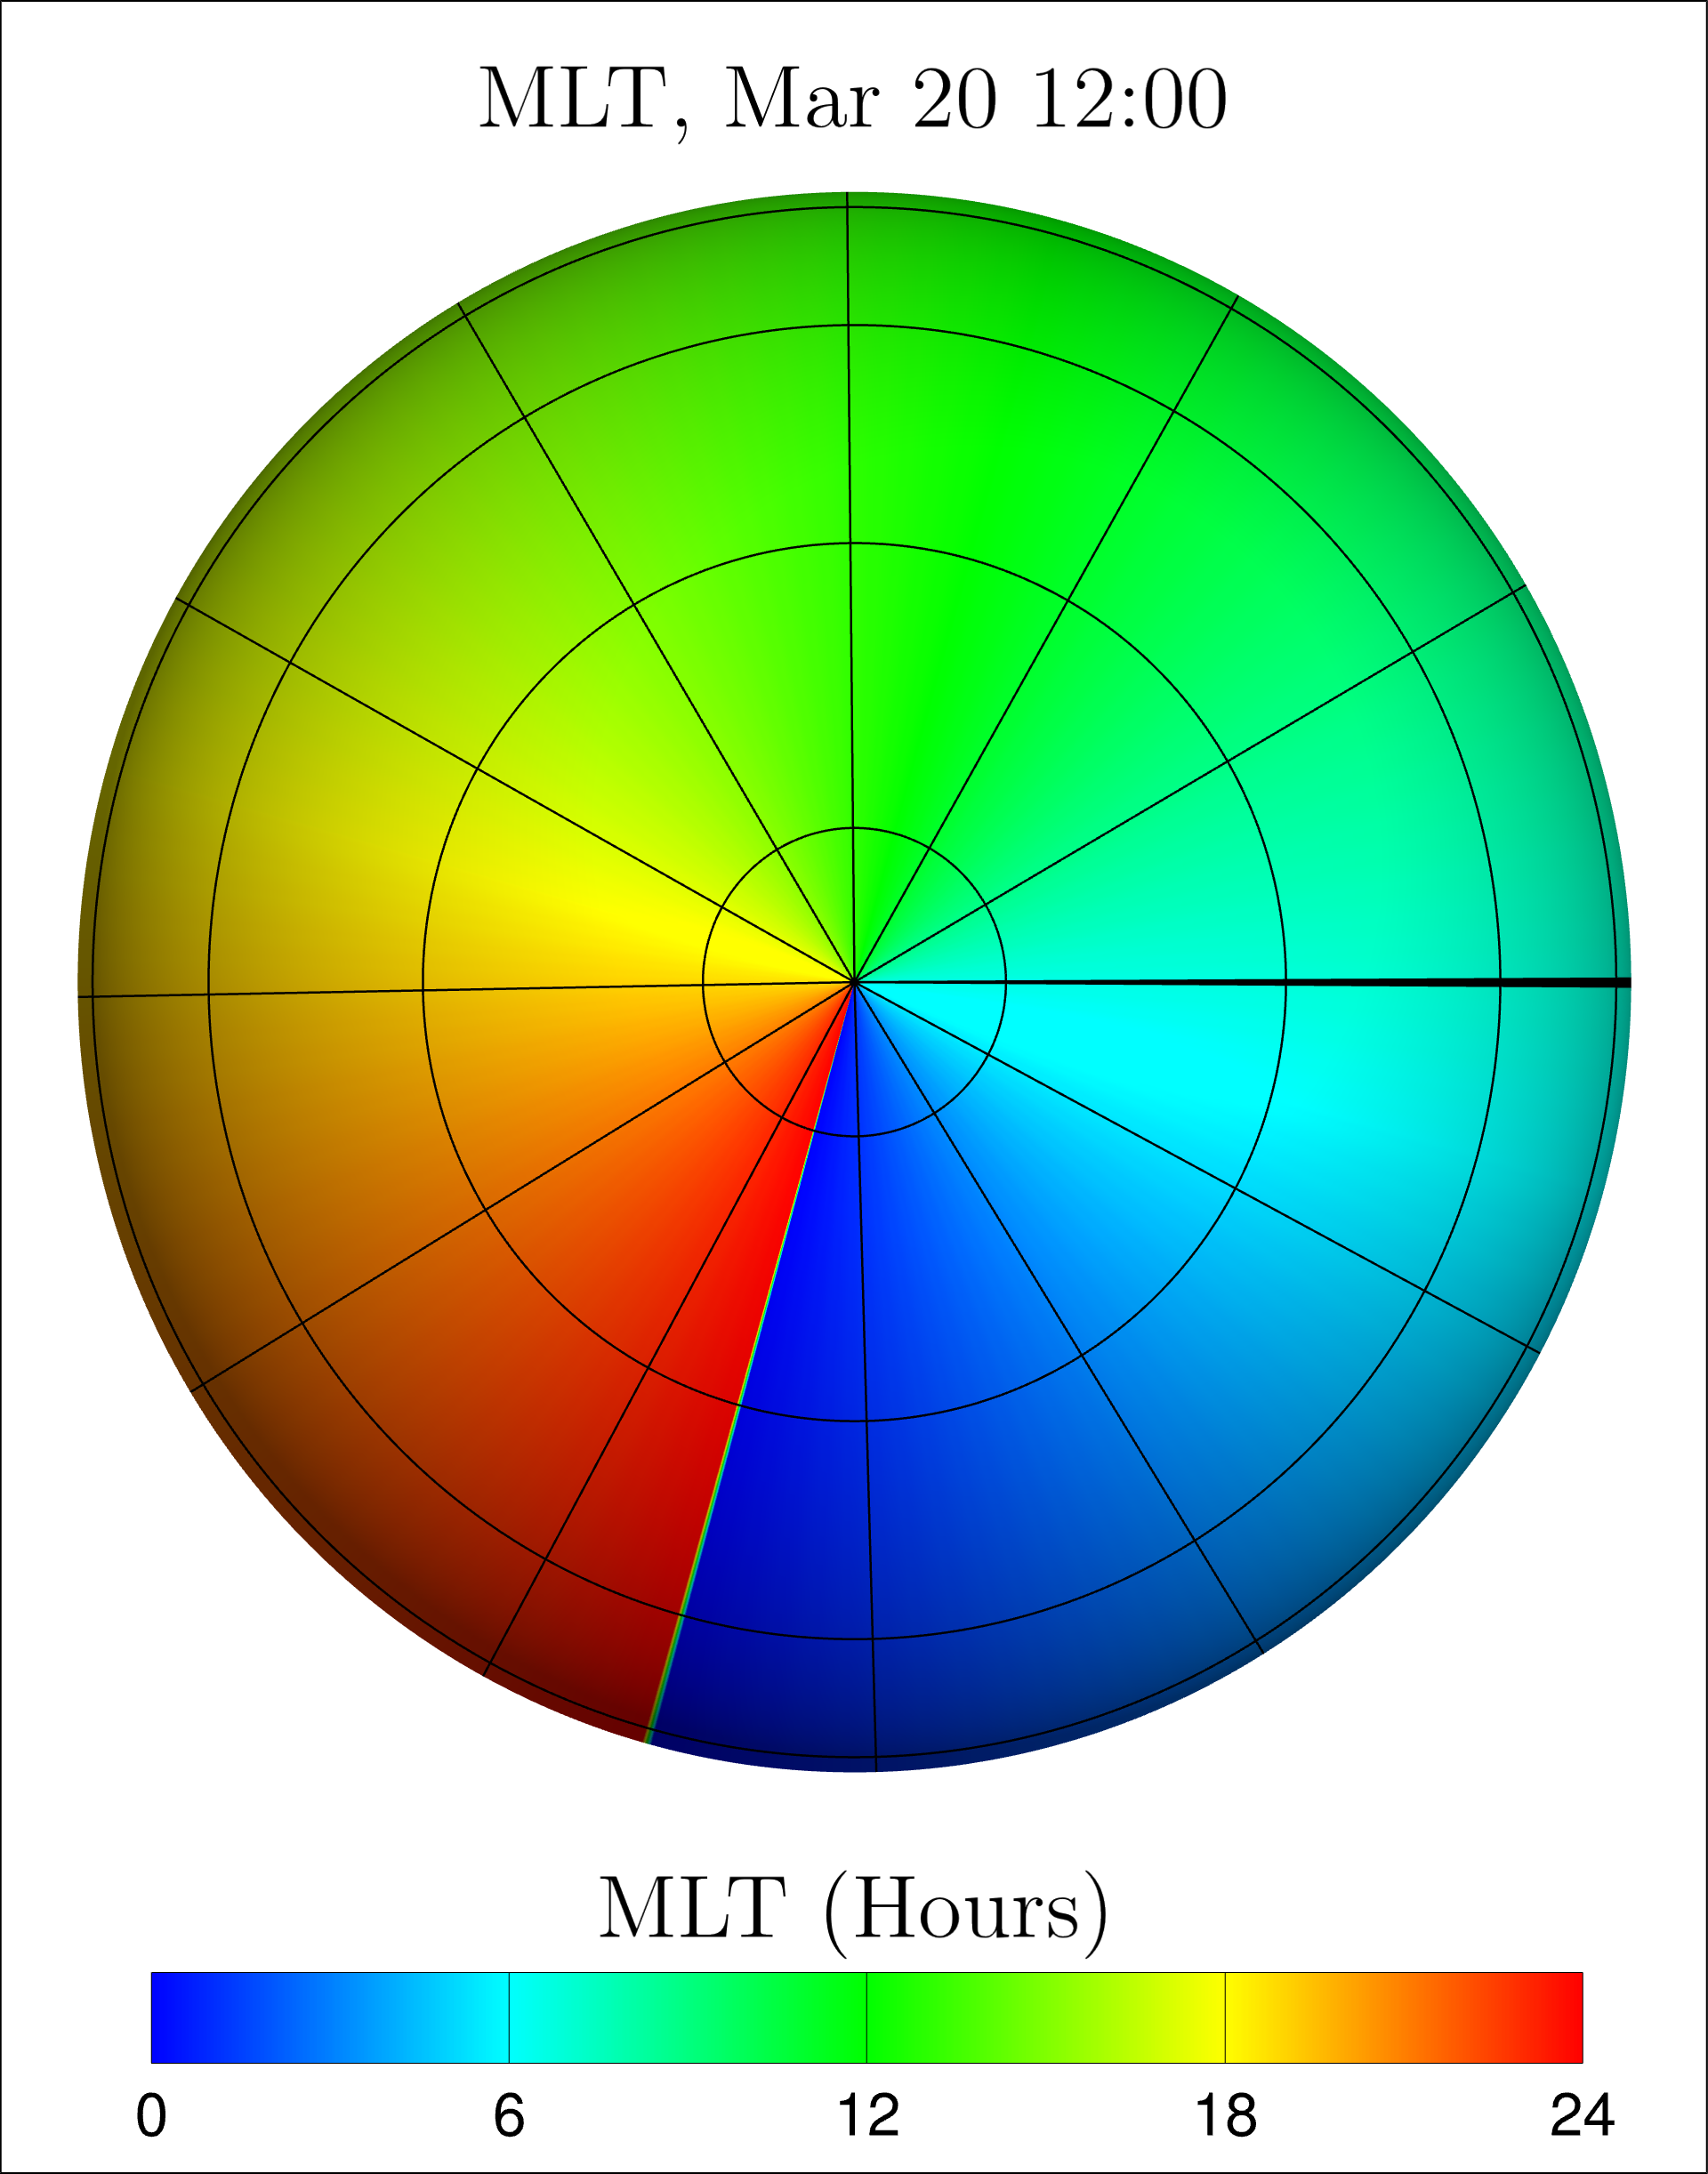
\includegraphics[width=0.4\textwidth]{figures/mltAlignment.png}
	\caption{Magnetic local time (MLT) in hours mapped onto the ionospheric sphere at equinox (Mar 20, 12:00).}
	\label{fig:mltAlignment}
\end{figure}
\section{Parallel Conductivity}
One large component that has been deferred from discussion so far is the parallel conductivity ($\sigz$). The parallel conductivity measures the conductivity along the magnetic field lines of the ionosphere. This is not widely available through empirical models as the Hall and Pedersen conductivity are. Therefore, the choice was made for the first iteration of this application to use the value $\sigz=1000\textrm{mhos}$. This serves as a reasonable stand in for the parallel conductivity due to the higher order of magnitude it exhibits~\citep{ionospheric_ridley_2003} relative to the Hall and Pederson conductivities. Future work is planned to investigate the feasibility of ionosphere models such as NRLMSIS~\citep{nrlmsis_emmert_2020} and IRI~\citep{international_bilitza_2022} to provide ion, electron and neutral densities. These could theoretically be used with the collision model in Equation~\ref{eq:physical_conduct} to derive all three conductivities from a first-principles approach. Further testing is required to verify the validity of this approach. This approach would allow for a value to be computed for the parallel conductivity, removing the need for the constant approximation.

\chapter{Numerical Implementation}
\label{chap:implementation}
\section{Coordinate Systems}
The ionosphere model that is presented in this paper is built in a spherical coordinate system. Spherical coordinates can be related to cartesian coordinates by the following equation:
\begin{equation}
	\bm r = \norm{\bm r}\left( \sin\theta\cos\phi, \sin\theta\sin\phi, \cos\theta\right)
	\label{eq:spherical_to_cartesian}
\end{equation}
There are two main benefits to using a spherical coordinate system for this problem. The first is the ability to use magnetic dipole coordinates as defined in~\citet{laundal2017}. This dipole coordinate system provides magnetic field orientation as a direct function of position, allowing the conductivity tensor that \citet{amm1996} presents (Equation~\ref{eq:conductivity_tensor}) to be utilized. The second is the ability to transform the coordinate system to geographic coordinates using a simple matrix rotation. This technique is discussed in~\citet{laundal2017}, and is required to calculate the relative sun-earth positions for extreme ultra violet (EUV) conductivity modeling.


\section{Discretization}
\label{sec:discretization}
Equation~\ref{eqn:continuity_eqn} can be combined with the conductivity tensor (Equation~\ref{eq:conductivity_tensor}) to produce Equation~\ref{eq:expanded_continuity_equation} as shown in~\citet{goodman1995} and~\citet{amm1996}. This provides a single equation relating the radial current to the ionospheric potential with coefficients containing the Hall, Pedersen and parallel conductivities in a spherical coordinate system.

\begin{equation}
	\begin{aligned}
		j_{R}(R_{E},\theta,\phi) & = \frac{1}{R_{E}^{2}} \Bigg[ \frac{\partial^{2}\psi}{\partial\theta^{2}} \frac{\Sigma_{0}\Sigma_{p}}{C}                                                                                                                                                                                             \\
		                         & \quad + \frac{\partial^{2}\psi}{\partial\phi^{2}} \left\{ \frac{1}{\sin^{2}\theta} \left( \Sigma_{p} + \frac{\Sigma_{H}^{2}\sin^{2}\epsilon}{C} \right) \right\}                                                                                                                                    \\
		                         & \quad + \frac{\partial\psi}{\partial\theta} \left\{ \frac{\partial}{\partial\theta} \left( \frac{\Sigma_{0}\Sigma_{p}}{C} \right) + \cot\theta\frac{\Sigma_{0}\Sigma_{p}}{C} + \frac{1}{\sin\theta}\frac{\partial}{\partial\phi} \left( \frac{\Sigma_{0}\Sigma_{H}\cos\epsilon}{C} \right) \right\} \\
		                         & \quad + \frac{\partial\psi}{\partial\phi} \left\{ \frac{\partial}{\partial\theta} \left( \frac{\Sigma_{0}\Sigma_{H}(-\cos\epsilon)}{C\sin\theta} \right) + \frac{1}{\sin^{2}\theta}\frac{\partial}{\partial\phi} \left( \Sigma_{p} + \frac{\Sigma_{H}^{2}\sin^{2}\epsilon}{C} \right) \right.       \\
		                         & \quad \left. + \frac{\Sigma_{0}\Sigma_{H}(-\cos\epsilon)\cot\theta}{C\sin\theta} \right\} \Bigg]_{R=R_{E}}
	\end{aligned}
	\label{eq:expanded_continuity_equation}
\end{equation}

For the majority of the points on the mesh, central-difference derivative discretizations were used as given in Equations~\ref{eq:first_order_discretization}~and~\ref{eq:second_order_discretization} (adapted to $\phi$ and $\theta$ from~\citet{William_H_Press1992-ps}).

\begin{align}
	\pdv{\psi}{\phi}(\theta,\phi) \approx \frac{\psi(\theta, \phi + \Delta\phi)- \psi(\theta, \phi - \Delta\phi)}{2\Delta \phi} &  & \pdv{\psi}{\theta} \approx \frac{\psi(\theta+ \Delta\theta,\phi)- \psi(\theta- \Delta\theta,\phi)}{2\Delta \theta}
	\label{eq:first_order_discretization}
\end{align}
\begin{align}
	\pdv[2]{\psi}{\phi}(\theta,\phi) \approx
	\frac{\psi(\theta, \phi + \Delta\phi) - 2\psi(\theta,\phi) + \psi(\theta, \phi - \Delta\phi)}{\Delta\phi^{2}}
	 &  &
	\pdv[2]{\psi}{\theta}(\theta,\phi) \approx
	\frac{\psi(\theta + \Delta\theta, \phi) - 2\psi(\theta,\phi) + \psi(\theta - \Delta\theta, \phi)}{\Delta\theta^{2}}
	\label{eq:second_order_discretization}
\end{align}

Figure~\ref{diag:std_five_point} displays the behaviour of these  discretizations and the five point stencil that is generated for each point in the mesh. This is shown for an example point in the low latitude region.
\begin{figure}[htbp]
	\centering
	\includestandalone[width=0.7\textwidth]{diagrams/LowLatGrid}
	\caption{Standard five-point stencil on the spherical grid. Displays the finite-difference contributions from the $\phi$ and $\theta$ derivative used in the general interior case.}
	\label{diag:std_five_point}
\end{figure}

The coefficients that contain a derivative in Equation~\ref{eq:expanded_continuity_equation} were computed using the same finite-difference stencils from Equations~\ref{eq:first_order_discretization} and~\ref{eq:second_order_discretization}. Since the conductivity values are known for every grid point, derivative matrices $D_\phi$ and $D_\theta$ were defined that include the contributions from the surrounding points. By ordering the elements on the mesh with a flattened index $i$, these derivatives were computed as follows:
\begin{align*}
	\left[\pdv{}{\theta} \left(\frac{\Sigma_0\sigp}{C}\right)\right]^{(i)} = \sum_{j=0}^{n_{\phi}n_{\theta}-1} D_\theta^{(i,j)} \left(\frac{\Sigma_0\sigp}{C}\right)^{(j)}
\end{align*}

Through this process, all of the coefficients were determined for every point on the mesh, allowing a coupled system to be assembled in Trilinos~\citep{TrilinosPaper}. This system was then solved iteratively as shown in Section~\ref{sec:solver}. The remaining piece of the discretization is the treatment of the boundaries imposed by the spherical coordinate system.
\section{Boundary Conditions}
\label{sec:polar_boundary}
The currents through which the magnetosphere couples with the ionosphere travel along the earth's magnetic field lines. Due to the structure of the earth's magnetic field, these field-aligned currents primarily enter the ionosphere in the high-latitude region. The continuity and accuracy of the system in the high latitude region is therefore paramount to the accuracy of the coupling. There are three distinct problems that arise when solving this equation on a spherical mesh, all occurring in the polar regions.
\begin{enumerate}
	\item In a standard spherical 2D mesh utilizing a $(\theta,\phi)$ coordinate system, a coordinate singularity naturally occurs at the poles as multiple $\phi$ values are mapped to the same point in physical space.
	\item The expanded continuity equation (Equation~\ref{eq:expanded_continuity_equation}) introduces terms of $\frac{1}{\sin\theta}$ that will approach infinity as the pole is approached. The coefficients overall do not diverge in the high latitude limit due to contributions from other terms, however the equation that describes the poles must take into account the numerical error that would be introduced by evaluating these $\sin\theta$ values at the poles. This can be done by either using a version of the equation that eliminates these terms in the polar limit or by not evaluating this equation at the poles entirely.
	\item The five-point finite-difference approximation breaks down as continuity over the pole requires the pole to calculate contributions from the surrounding ring of points of the pole, not just four adjacent points.
\end{enumerate}
Due to these issues, a more complex boundary condition is required at the poles. The implemented boundary condition leveraged the 2D divergence theorem to generate a finite-volume style stencil for the polar point. This is detailed in the next section.

\subsection{Polar Cap Finite-Volume Boundary Condition}
To determine an accurate potential at the pole, there must be continuity of the potential when approaching from any direction. It follows that any equation that relates the pole potential to the surrounding region must take into account all of the adjacent grid points shown in Figure~\ref{diag:pole_behaviour_grid}.

\begin{figure}[htbp]
	\centering
	\begin{subfigure}[t]{0.48\textwidth}
		\centering
		\includestandalone[width=\textwidth]{diagrams/CapBC1}
		\caption{Pole point and adjacent grid points.}
		\label{diag:pole_behaviour_grid}
	\end{subfigure}
	\hfill
	\begin{subfigure}[t]{0.48\textwidth}
		\centering
		\includestandalone[width=\textwidth]{diagrams/CapBC2}
		\caption{Pole cap region $\C$ and its boundary $\parC$ indicated on the grid.}
		\label{diag:pole_behaviour_grid_cap}
	\end{subfigure}
	\caption{Grid structure in the polar region. The polar cap region $\C$ is introduced at radius $\Delta\theta/2$ to apply an accurate boundary condition.}
\end{figure}

The polar divergence theorem boundary condition achieves this through defining a region of radius $\Delta\theta/2$ around the pole and then applying the divergence theorem to Equation~\ref{eqn:continuity_eqn} converting the expression to a line integral around the pole. Figure~\ref{diag:pole_behaviour_grid_cap} displays this region. This equation relates the values on the boundary $\parC$ to the total radial current passing through the $\C$ region as shown in Equation~\ref{eq:pole_integration_line2}.
\begin{equation}
	\iint_{\C} j_R(R_e) dA  =\iint_{\C}  \left[\nabla_\perp\cdot (\Sigma\cdot \nabla \psi)_\perp\right]dA
	\implies J_{cap}=\oint_{\parC}\left[(\Sigma\cdot \nabla \psi)_\perp\right]dl
	\label{eq:pole_integration_line2}
\end{equation}
$J_{\rm cap}$ provides the total current entering the region $\C$ in Figure~\ref{diag:pole_behaviour_grid_cap}. In practice, it is calculated by assuming that the polar current density $j_{R,pole}$ is representative of the average current density over the $\C$ region.
\begin{equation}
	J_{\rm cap} = j_{R,pole}\cdot A_\C = j_{R,pole}\cdot 2\pi R_E^2(1 -\cos\theta_{\parC})
\end{equation}
By evaluating the inner $\Sigma \cdot \nabla \psi$ expression in Equation~\ref{eq:pole_integration_line2} with the conductivity tensor in spherical coordinates and simplifying, Equation~\ref{eq:pole_integration_exp} is produced.
\begin{equation}
	J_{\rm cap} = \int_{0}^{2\pi}\left[\sin\theta_{\parC}\cdot
		\frac{\partial \psi}{\partial \theta}(\theta_{\parC}, \phi)\cdot
		\Sigma_{\theta\theta} (\theta_{\parC},\phi)\pm
		\frac{\partial\psi}{\partial\phi}(\theta_{\parC},\phi)\cdot
		\Sigma_{\theta\phi}(\theta_{\parC},\phi)
		\right] d\phi
	\label{eq:pole_integration_exp}
\end{equation}

Where $\theta_{\parC}=\Delta\theta/2$ and $\theta_0=\pi -\Delta\theta/2$ on the north and south pole respectively. The central sum is positive on the north pole and negative on the south pole due to the opposite direction of the normal vector to $\parC$ relative to $\hat\theta$ in the north and south poles.

\subsubsection{Discretization}
In this section a superscript of $(i,j)$ denotes evaluation at the grid point located at $(\theta_i,\phi_j)$. $(a,i)$ is used to denote evaluation on the adjacent points to the north pole as shown in Figure~\ref{diag:pole_behaviour_grid} for longitude $\phi_i$. $(\parC, i)$ is used to denote evaluation for a grid point on the polar cap boundary $\parC$ with the longitude $\phi_i$. The rest of the derivation will assume the north pole case with a positive normal.


To determine a linear representation of Equation~\ref{eq:pole_integration_exp} the first step involves discretizing the term obtained by the divergence theorem using a Riemann sum approximation, providing Equation~\ref{eq:fully_disc_pole}.
\begin{equation}
	J_{\rm cap} \approx\sum_{i=0}^{n_{\phi}-1}
	\left[
		\sin\theta_{\parC} \cdot \Sigma_{\theta\theta}^ {(\parC,i)}\cdot\frac{\partial \psi}{\partial \theta}^{(\parC,i)}+
		\Sigma_{\theta\phi}^{(\parC,i)}\cdot\frac{\partial\psi}{\partial\phi}^{(\parC,i)}
		\right] \Delta\phi
	\label{eq:fully_disc_pole}
\end{equation}
To create a linear equation containing the potential at the pole $\psi^{(\rm pole)}$ as a function of other grid points, the terms that are on $\parC$ must be eliminated from the equation. The $\theta$ derivative term is discretized using the standard first-derivative discretization with a denominator of $\Delta\theta$ due to $\parC$ being only $\Delta\theta/2$ from the pole (Equation~\ref{eq:first_order_discretization}). This introduces the pole into the equation and removes terms on the boundary $\parC$.
\begin{equation}
	\frac{\partial \psi}{\partial \theta}^{(\parC,i)}
	\approx \frac{\psi^{(\rm pole)} - \psi^{(a, i)}}{\Delta \theta}
\end{equation}
The discretized expansion can not be applied however to the $\phi$ derivative, since this would not remove the points on the boundary $\parC$. Therefore a different approach is required. The $\pdv{\psi}{\phi}$ term can be expanded into a Cartesian coordinate system by first applying the multi-variable chain rule.
\begin{equation*}
	\pdv{\psi}{\phi} =
	\pdv{\psi}{x}\pdv{x}{\phi}
	+ \pdv{\psi}{y}\pdv{y}{\phi}
	+\pdv{\psi}{z}\pdv{z}{\phi} = \bm\nabla \psi \cdot \pdv{\bm r}{\phi}
\end{equation*}
The $\hat\phi$ unit vector's direction can be determined with the following equation:
\begin{equation}
	\hat\phi = \left(-\sin\phi, \cos\phi, 0\right)
	\label{eq:phi_unit_vector}
\end{equation}
The $\pdv{\bm r}{\phi}$ term can be expanded by applying the spherical to Cartesian coordinate transformation Equation~\ref{eq:spherical_to_cartesian} for the mesh's radius of $R_E$ and applying the $\phi$ unit vector definition (Equation~\ref{eq:phi_unit_vector}) to simplify.
\begin{equation*}
	\pdv{\bm r}{\phi} = R_E\pdv{\phi} \left( \sin\theta\cos\phi, \sin\theta\sin\phi, \cos\theta\right) = R_E\sin\theta\left( -\sin\phi, \cos\phi,0 \right) = R_E\sin\theta\hat\phi
\end{equation*}
This provides the following expression for the $\phi$ derivative.
\begin{equation*}
	\pdv{\psi}{\phi} = \bm\nabla\psi \cdot R_E\sin\theta\hat\phi
\end{equation*}
Since $||\hat\phi|| = 1$ by definition, by the Cauchy–Schwarz inequality, $|\bm\nabla\psi \cdot \hat\phi| \le ||\bm\nabla\psi||\cdot  ||\hat\phi||= \norm{\bm\nabla\psi}$ which provides an upper bound on the absolute value of $\pdv{\psi}{\phi}$.
\begin{equation*}
	\abs{\pdv{\psi}{\phi}} = \abs{R_E\sin\theta (\bm\nabla\psi\cdot\hat\phi)}=\abs{R_E\sin\theta}\cdot \abs{\bm\nabla\psi\cdot \hat\phi} \le \abs{R_E\sin\theta}\cdot \norm{\bm\nabla\psi}
\end{equation*}
For a continuous electric field, the norm $\norm{\bm\nabla\psi}$ must be finite across all of the points on the mesh. Therefore it follows that in the limit of $\theta\rightarrow0$, the $\sin\theta$ term dominates resulting in the following expression.
\begin{equation*}
	\lim_{\theta\rightarrow0}\left|\pdv{\psi}{\phi}\right| = \lim_{\theta\rightarrow0} \left(\abs{R_E\sin\theta}\cdot \norm{\bm\nabla\psi}\right) = 0
\end{equation*}
Therefore, it follows that the $\phi$ derivative must go from a generally nonzero value at the adjacent grid points $\theta_a$ to zero at the pole. To approximate the value of the derivative at the midpoint $\parC$ between these points, a linear interpolation is performed and the Equation~\ref{eq:first_order_discretization} first-derivative central-difference approximation was applied to the resulting term:
\begin{equation}
	\frac{\partial \psi}{\partial \phi}^{(\parC,i)}
	\approx \frac{1}{2}\left(\pdv{\psi}{\phi}^{(a, i)} + \pdv{\psi}{\phi}^{(\rm pole)} \right) = \frac12\pdv{\psi}{\phi}^{(a,i)}
	\approx \frac{\psi^{(a, i+1)} - \psi^{(a, i-1)}}{4\Delta \phi}
\end{equation}
By performing a similar average on the conductivity values, a fully linear equation containing only points on the adjacent latitude ring and the pole itself can be obtained in Equation~\ref{eq:fully_disc_pole2}.

\begin{equation}
	\begin{aligned}
		J_{\rm cap} \approx\sum_{i=0}^{n_{\phi}-1}
		 & \left[
			\sin\theta_0\cdot
			\frac{\Sigma^{(a, i)}_{\theta\theta} + \Sigma^{(\rm pole)}_{\theta\theta}}{2}\cdot
			\frac{\psi^{(\rm pole)} - \psi^{(a, i)}}{\Delta \theta}\ +
		\right.                                                                                     \\
		 & \ \ \left.\frac{\Sigma^{(a, i)}_{\theta\phi} + \Sigma^{(\rm pole)}_{\theta\phi}}{2}\cdot
			\frac{\psi^{(a, i+1)} - \psi^{(a, i-1)}}{4\Delta \phi}
			\right] \Delta\phi
		\label{eq:fully_disc_pole2}
	\end{aligned}
\end{equation}
Equation~\ref{eq:fully_disc_pole2} provides a row in the linear system that couples the pole point to all of the $n_\phi$ adjacent points on the next latitude ring, maintaining continuity of the solution. Figure~\ref{fig:boundary_condition_contour} shows the behaviour of the potential solution from the ionosphere model at the pole, exhibiting continuous contour lines.

With the boundary condition, the linear system is complete. Section~\ref{sec:solver} describes the iterative methods used to solve the system.
\begin{figure}[H]
	\centering
	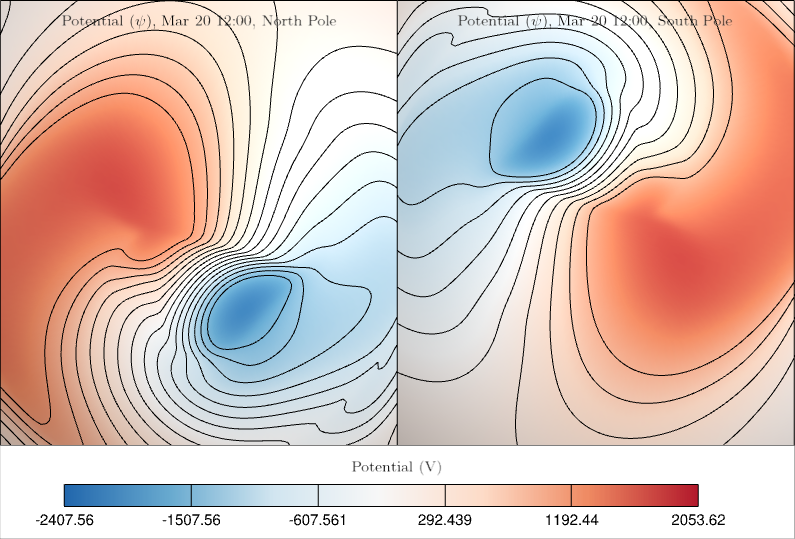
\includegraphics[width=0.7\textwidth]{figures/boundary condition zoomed.png}
	\caption{Boundary condition behaviour for an example southward interplanetary magnetic field solve showing continuous contour lines over the poles. }
	\label{fig:boundary_condition_contour}
\end{figure}

\section{Solver}\label{sec:solver}
In Sections~\ref{sec:discretization} and~\ref{sec:polar_boundary} a linear system of equations was produced to accurately model ionosphere electrodynamics for the magnetosphere-ionosphere coupling problem by solving Equation~\ref{eqn:continuity_eqn} on a 2D shell approximation of the ionosphere. In order to solve this system, the Trilinos~\citep{TrilinosPaper} C++ framework was used to build an MPI-parallel solver. This section will explore the different packages that were used and the implementation details of an iterative solve of this system.

\subsection{Trilinos Packages}
\subsubsection{Tpetra}
The coupled system that was generated from the combination of the five point stencil interior points and the polar divergence condition polar points was stored in Tpetra~\citep{TpetraPaper}. Tpetra provides a standard interface that allows a consistent representation for mathematical objects such as vectors and matrices in a wide array of modern Trilinos packages. Tpetra is also used to manage the distribution of vector and matrix elements between MPI ranks through a common interface known as a \texttt{Tpetra::Map}. This allows the ability to tweak the distribution on a global scale by changing a single \texttt{Tpetra::Map} instance. In this application, a sequential contiguous block of rows in $\phi$-major order was provided to each rank. However, potentially exploring different distribution strategies such as interleaved row storage between ranks or using the Zoltan~\citep{ZoltanUsersGuide} framework could potentially improve the performance of the application further and this is planned to be explored in the future.
\subsubsection{Belos}
Belos~\citep{BelosPaper} is an iterative solver library in Trilinos that provides a number of iterative solvers with configurable parameters. Belos provides a \texttt{Belos::SolverFactory} class that enables swapping solvers for performance analysis on the fly. A runtime analysis on the system was performed to determine the improved solver choice and configuration settings for this problem and this is detailed in Section~\ref{sec:convergence_study}. In the end a \texttt{GMRES} solver with preconditioning was used as this showed the highest performance on the matrix generated by this problem. The Belos solver and the associated solver parameters are configurable from a YAML configuration file that is passed into the application as a command line argument. This allows for easy solver and parameter performance studies and tuning without requiring re-compilation of the application.
\subsubsection{Preconditioning}
Two preconditioning strategies were explored in this problem. MueLu~\citep{MueLuUsersGuide} provides multi-grid preconditioning and solvers implemented using the Tpetra interface. IfPack2 is also included within the application and provides incomplete lower upper triangularization preconditioning methods. Similarly to the Belos solver, the preconditioner for the problem and its associated parameters are configurable through the YAML configuration file. This provides a single configuration file that can be used to tune the performance of the preconditioner for this problem. Section~\ref{sec:convergence_study} contains suggested values for the preconditioner that were found to be well performing through empirical testing.
\subsection{Application Structure}
\label{sec:application_structure}
The core of the configurability of this solver is the YAML configuration file that can be passed as a command line argument to the application. The boundary condition and equation can be configured through this file. While the current application only offers the use of the continuity equation Equation~\ref{eqn:continuity_eqn} from~\citet{goodman1995} with the conductivity tensor provided by~\citet{amm1996} combined with the boundary condition discussed in Section~\ref{sec:polar_boundary}, there are plans to extend these capabilities. Specifically, there is an alternative boundary condition that is in the process of implementation that utilizes a ``ghost ring'' approach to estimate the value at the pole using multiple five point stencils at a small distance from the pole and averages them. Additionally, incorporating the original conductivity tensor provided by~\citet{goodman1995} is also being explored as this will provide a conductivity tensor that does not require the approximation of the parallel conductivity as described in Chapter~\ref{chap:conductivity}.

\begin{figure}[htbp]
	\centering
	\includestandalone[width=\textwidth]{diagrams/SolverDiagram}
	\caption{Application structure diagram displaying the data flow of the solver and the configurable YAML parameters. Solid lines indicate the flow of computed parameters while the dashed lines display the configuration parameters. Conductivity tensor $\Sigma$ shows incoming data from the conductivity model described in Chapter~\ref{chap:conductivity}. The full application diagram is shown in Figure~\ref{diag:full_flow2}.}
	\label{diag:solver_flow}
\end{figure}
Figure~\ref{diag:solver_flow} displays the solver application structure from a high level view, and from this, the main solver loop can be clearly seen. The application will take in the interpolated MHD field aligned current data mapped down to the ionosphere; use that to generate the associated matrix, source term and initial guess based on the equation structure and boundary condition provided by the YAML file; then it will proceed to apply the preconditioner and solver to the problem, returning the potential to the MHD model to close the magnetospheric currents.

The MHD interpolation is currently in progress as indicated in Figure~\ref{diag:solver_flow} and therefore the figures in Chapter~\ref{chap:results} are generated using a pre-interpolated source term that was produced by the ionosphere model used in~\citet{global_groth_2000}. Once the coupling is complete, this circular loop structure will allow the application to run in parallel with the MHD code, receiving updated radial currents, over multiple MHD time-steps, piped into the application. This will allow the application to retain matrix structure through iterations. The feasibility of this is dependent on the timescale involved due to the conductivity being dependent on date and time, however this could potentially reduce the solve time as discussed in Section~\ref{sec:convergence_study}.

\section{Runtime Analysis and Solver Optimization}
\label{sec:convergence_study}
A short convergence speed study was performed on the model to determine parameters for the preconditioner and Belos solver to improve the performance. This was performed on a grid with size $n_\phi = 512$ and $n_\theta=256$. As discussed in Section~\ref{sec:solver}, both MueLu and IfPack2 preconditioners were tested to determine the best-performing configuration for the application. This was done in two stages. The first stage involved running the simulation on the same source input, testing different preconditioners and solvers while sweeping through their parameters. In the second stage, a convergence analysis was performed on the best resulting configuration for IfPack2 ILU preconditioning and the best resulting configuration with the MueLu preconditioning for a more comprehensive comparison.
\subsection{Parameter Sweep}
\label{sec:parameter_sweep}
For this stage of the experiment, two preconditioning packages were examined. The first using algebraic multi-grid provided by MueLu as a preconditioner with the \texttt{RILUK} solver used as a smoother and coarse solver, and the second using IfPack2 with \texttt{RILUK}. \texttt{RILUK} is the Trilinos implementation for ILU factorization. These preconditioners were found to have the best performance from the MueLu and Ifpack2 packages on this problem at default settings and therefore were selected for further testing. The \texttt{GMRES} solver from Belos was used as the solver for the problem and was chosen similarly as it was the Belos solver that produced the fastest runtime on this problem at default settings. Table~\ref{tab:sweep_riluk} shows the parameters that were tested for the IfPack2 ILU preconditioning and Table~\ref{tab:sweep_muelu} shows the parameters that were tested for the MueLu preconditioning. All tests were performed on a linux workstation with an \textbf{AMD Ryzen 5800x 8-core processor} with 16 threads available through simultaneous multithreading and 32GB of \textbf{DDR4 RAM}. Runtime was compared using the wall-clock runtime for the solver section of the application for one run of each of the configurations.
\begin{table}[H]
	\centering
	\begin{minipage}{0.48\textwidth}
		\centering
		\begin{tabular}{ll}
			\toprule
			\textbf{Parameter} & \textbf{Values}  \\
			\midrule
			Fill Level         & 2, 5, 10, 15, 20 \\
			Num Blocks         & 100, 200, 500    \\
			Processor Count    & 2, 4, 8, 14      \\
			\bottomrule
		\end{tabular}
		\captionof{table}{Ifpack2 RILUK sweep configurations}
		\label{tab:sweep_riluk}
	\end{minipage}
	\hfill
	\begin{minipage}{0.48\textwidth}
		\centering
		\begin{tabular}{ll}
			\toprule
			\textbf{Parameter}  & \textbf{Values} \\
			\midrule
			Smoother Fill Level & 1, 2, 4         \\
			Num Blocks          & 100, 200, 500   \\
			Processor Count     & 2, 4, 8, 14     \\
			\bottomrule
		\end{tabular}
		\captionof{table}{MueLu sweep configurations}
		\label{tab:sweep_muelu}
	\end{minipage}
\end{table}
This resulted in 60 configurations tested for the IfPack2 preconditioner and 24 for the MueLu preconditioner. The 14 processor runs were included in this analysis, however due to the simultaneous multi-threading on the CPU it is not possible to assign 14 physical cores to the problem. The runs for processor count of 14 are therefore likely not as indicative of scaling performance of this application. The raw results of this analysis are summarized in Tables~\ref{tab:ifpack_results} and \ref{tab:muelu_results} for the RILUK and MueLu preconditioners respectively. The fastest runtime for IfPack2 was achieved with 500 for num blocks in GMRES and a level of fill of 10 for ILUK on 8 processors. The best performing MueLu configuration was GMRES with a \texttt{num blocks} of 100 and a smoother fill level of 4 on 8 processors. These configurations were then selected for a more in depth convergence study as detailed in Section~\ref{sec:convergence_analysis}.
\subsection{Convergence Analysis}
\label{sec:convergence_analysis}
For the convergence analysis, the best performing algorithms from Section~\ref{sec:parameter_sweep} were run 10 times each on 2, 4, 8 and 14 processors. Multiple metrics were tracked throughout the simulation including the wall-clock time for conductivity computation and solver setup and computation. Additionally the iteration counts were recorded as well as the relative residual per iteration. Figures~\ref{fig:scaling_time} and~\ref{fig:scaling_iters} display the scaling behaviour of the algorithm iteration count and solve time (wall clock time between starting preconditioner setup and solver completion).
\begin{figure}[ht]
	\centering
	\begin{subfigure}[t]{0.45\textwidth}
		\centering
		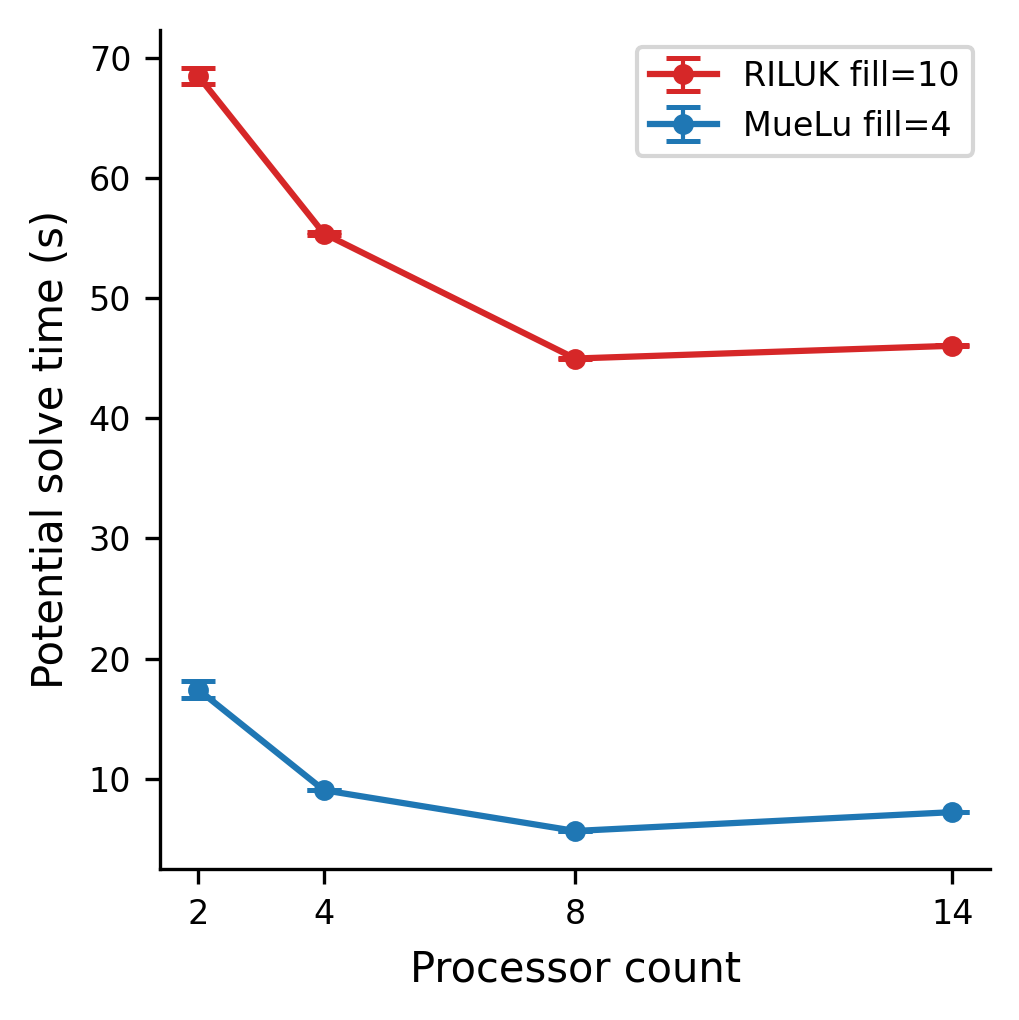
\includegraphics[width=\textwidth]
		{../convergenceAnalysis/plotsAndData/optimalRun/scaling_time_errorbars.png}
		\caption{Wall clock solve time for the coupled potential system for the MueLu and RILUK algorithms vs processor count.}
		\label{fig:scaling_time}
	\end{subfigure}
	\hfill
	\begin{subfigure}[t]{0.45\textwidth}
		\centering
		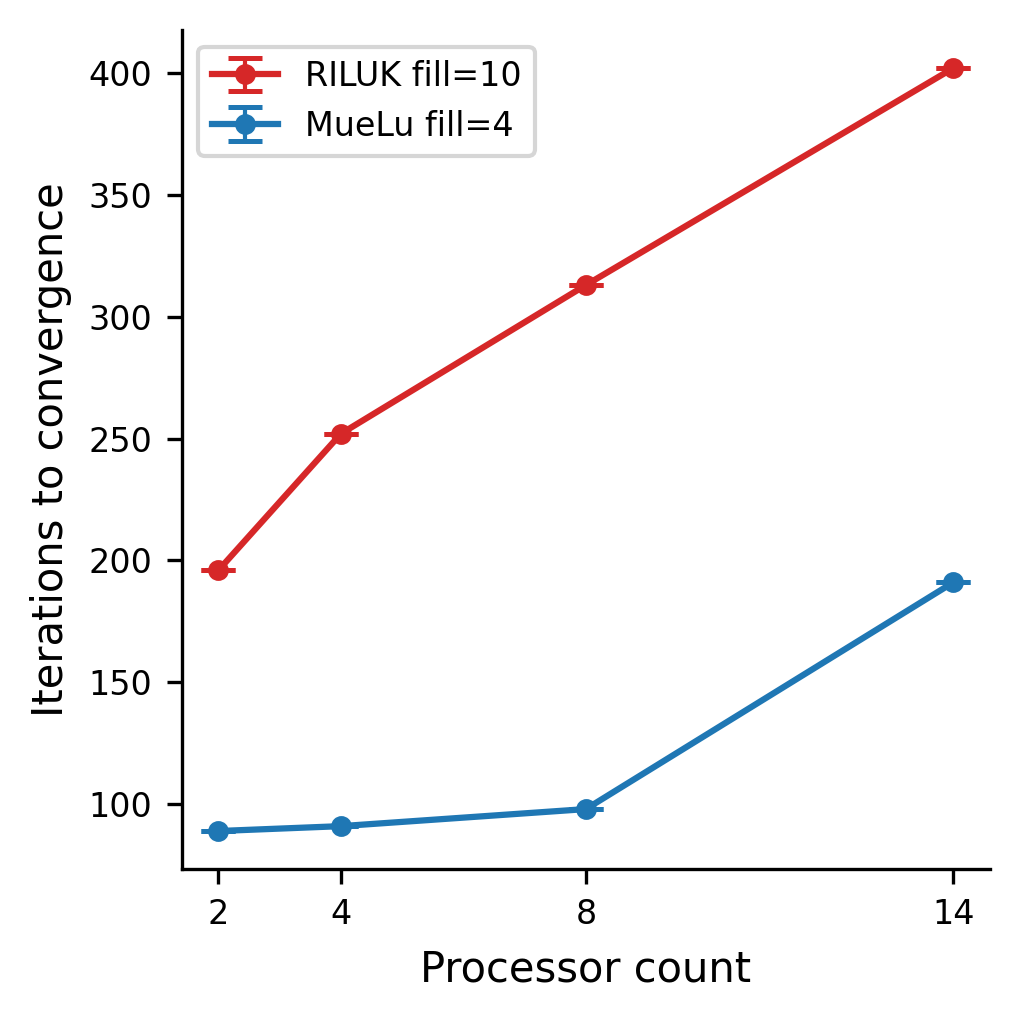
\includegraphics[width=\textwidth]
		{../convergenceAnalysis/plotsAndData/optimalRun/scaling_iterations_errorbars.png}
		\caption{Number of iterations to solve the coupled potential system for the MueLu and RILUK algorithms vs processor count.}
		\label{fig:scaling_iters}
	\end{subfigure}
	\caption{Application scaling behaviour for the IfPack2 and MueLu preconditioners across increasing processor counts, averaged over the 10 runs.}
	\label{fig:scaling_time_iters}
\end{figure}

Figure~\ref{fig:scaling_time} compares the wall-clock runtime for the two preconditioners. It can be clearly seen that the MueLu's algebraic multi-grid produced significantly faster results. Notably, the increase in performance from 2 to 4 processors is relatively significant, however the improvement from 4 to 8 is notably reduced, especially for the MueLu preconditioner. In both algorithms, the solve time of the 14 processor runs was slower than the 8 processor runs. This scaling behaviour could be due to increasing communication requirements between MPI ranks but more comprehensive testing on a dedicated network with more than 8 cores would be required to verify this. Figure~\ref{fig:scaling_iters} shows the iteration count required to reach the $1\times10^{-6}$ relative residual target. The IfPack2 preconditioner showed a rapid increase in iteration count from 2 to 14 processors, whereas the MueLu iteration count remained much more stable between 2 and 8 processors, only increasing in the 14 processor case.

Figure~\ref{fig:scaling_wallclock} shows the total runtime of both preconditioner configurations. It shows a similar trend to the results shown in the figures in~\ref{fig:scaling_time_iters}. This shows the minimal effect that the conductivity overhead has on the application runtime.
\begin{figure}[H]
	\centering
	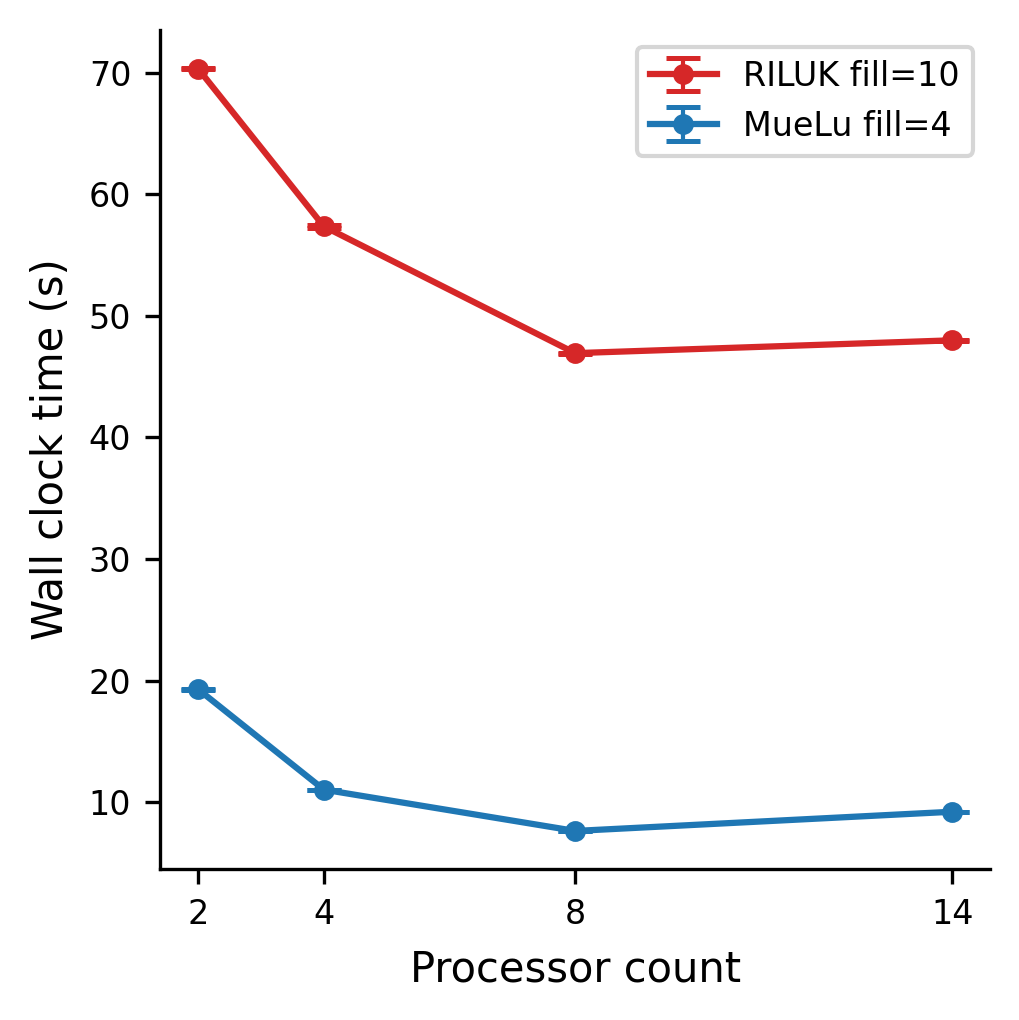
\includegraphics[width=0.45\textwidth]
	{../convergenceAnalysis/plotsAndData/optimalRun/scaling_wallclock_errorbars.png}
	\caption{Total wall clock time for the application solve portion for the IfPack2 and MueLu preconditioners vs processor count averaged over the 10 runs.}\label{fig:scaling_wallclock}
\end{figure}


\begin{figure}[ht]
	\centering
	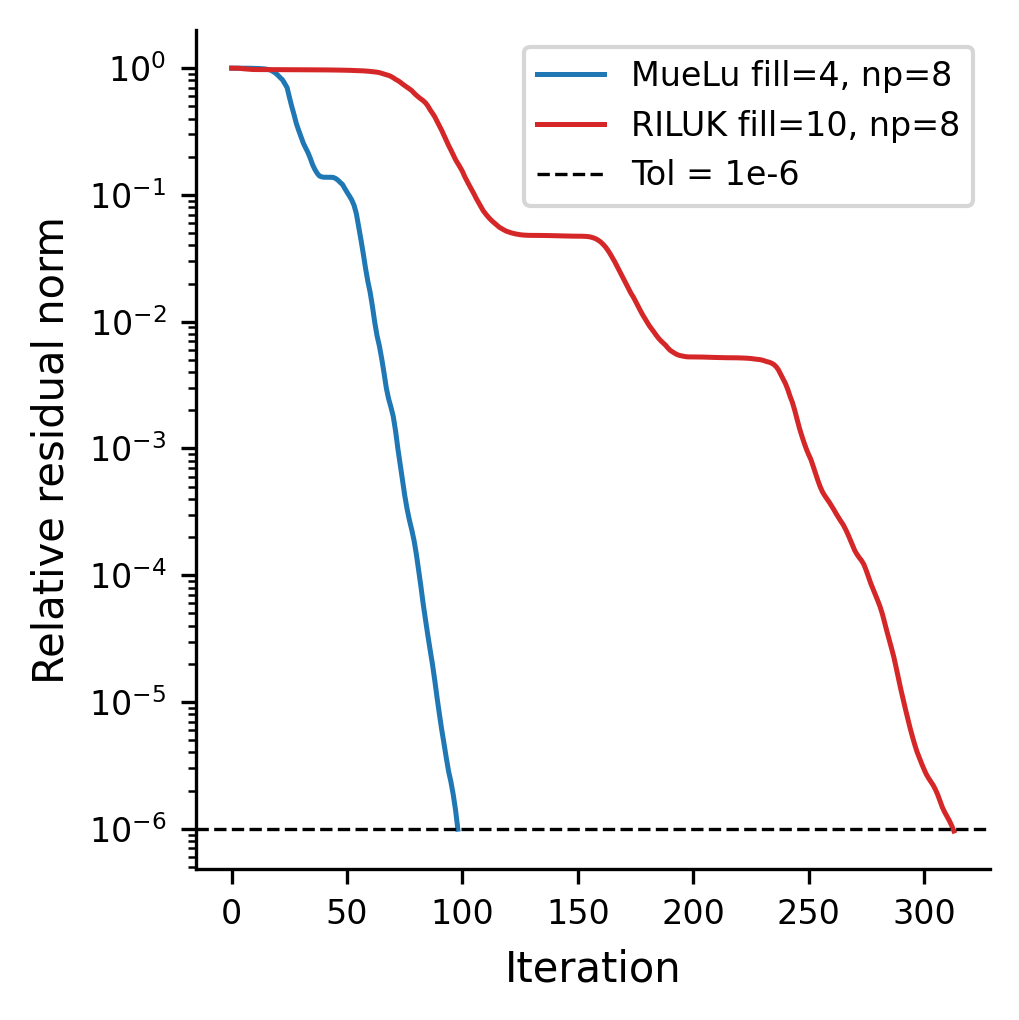
\includegraphics[width=0.45\textwidth]
	{../convergenceAnalysis/plotsAndData/optimalRun/convergence_curves.png}
	\caption{Convergence plot for the IfPack2 (\texttt{RILUK}) preconditioner vs the MueLu preconditioner. Shows relative residual (logarithmic) vs iteration count with the $1\times10^{-6}$ convergence tolerance displayed. Averaged over the 10 runs.}
	\label{fig:convergence_curves}
\end{figure}
In Figure~\ref{fig:convergence_curves} the convergence behaviour of both preconditioners can be seen averaged over the 10 runs. The IfPack2 preconditioner showed clear stalling behaviour at multiple iteration levels which was clearly reduced with the MueLu preconditioner. Overall, the convergence behaviour of the MueLu preconditioner showed largely improved results over just using \texttt{RILUK} provided by IfPack2 on this problem.

Figure~\ref{fig:time_breakdown} displays the time breakdown between the different sections of the application averaged over the 10 runs of the application. This shows the significant portion of application runtime that is dedicated to the solve procedure itself and the importance of solver optimization.
\begin{figure}[H]
	\centering
	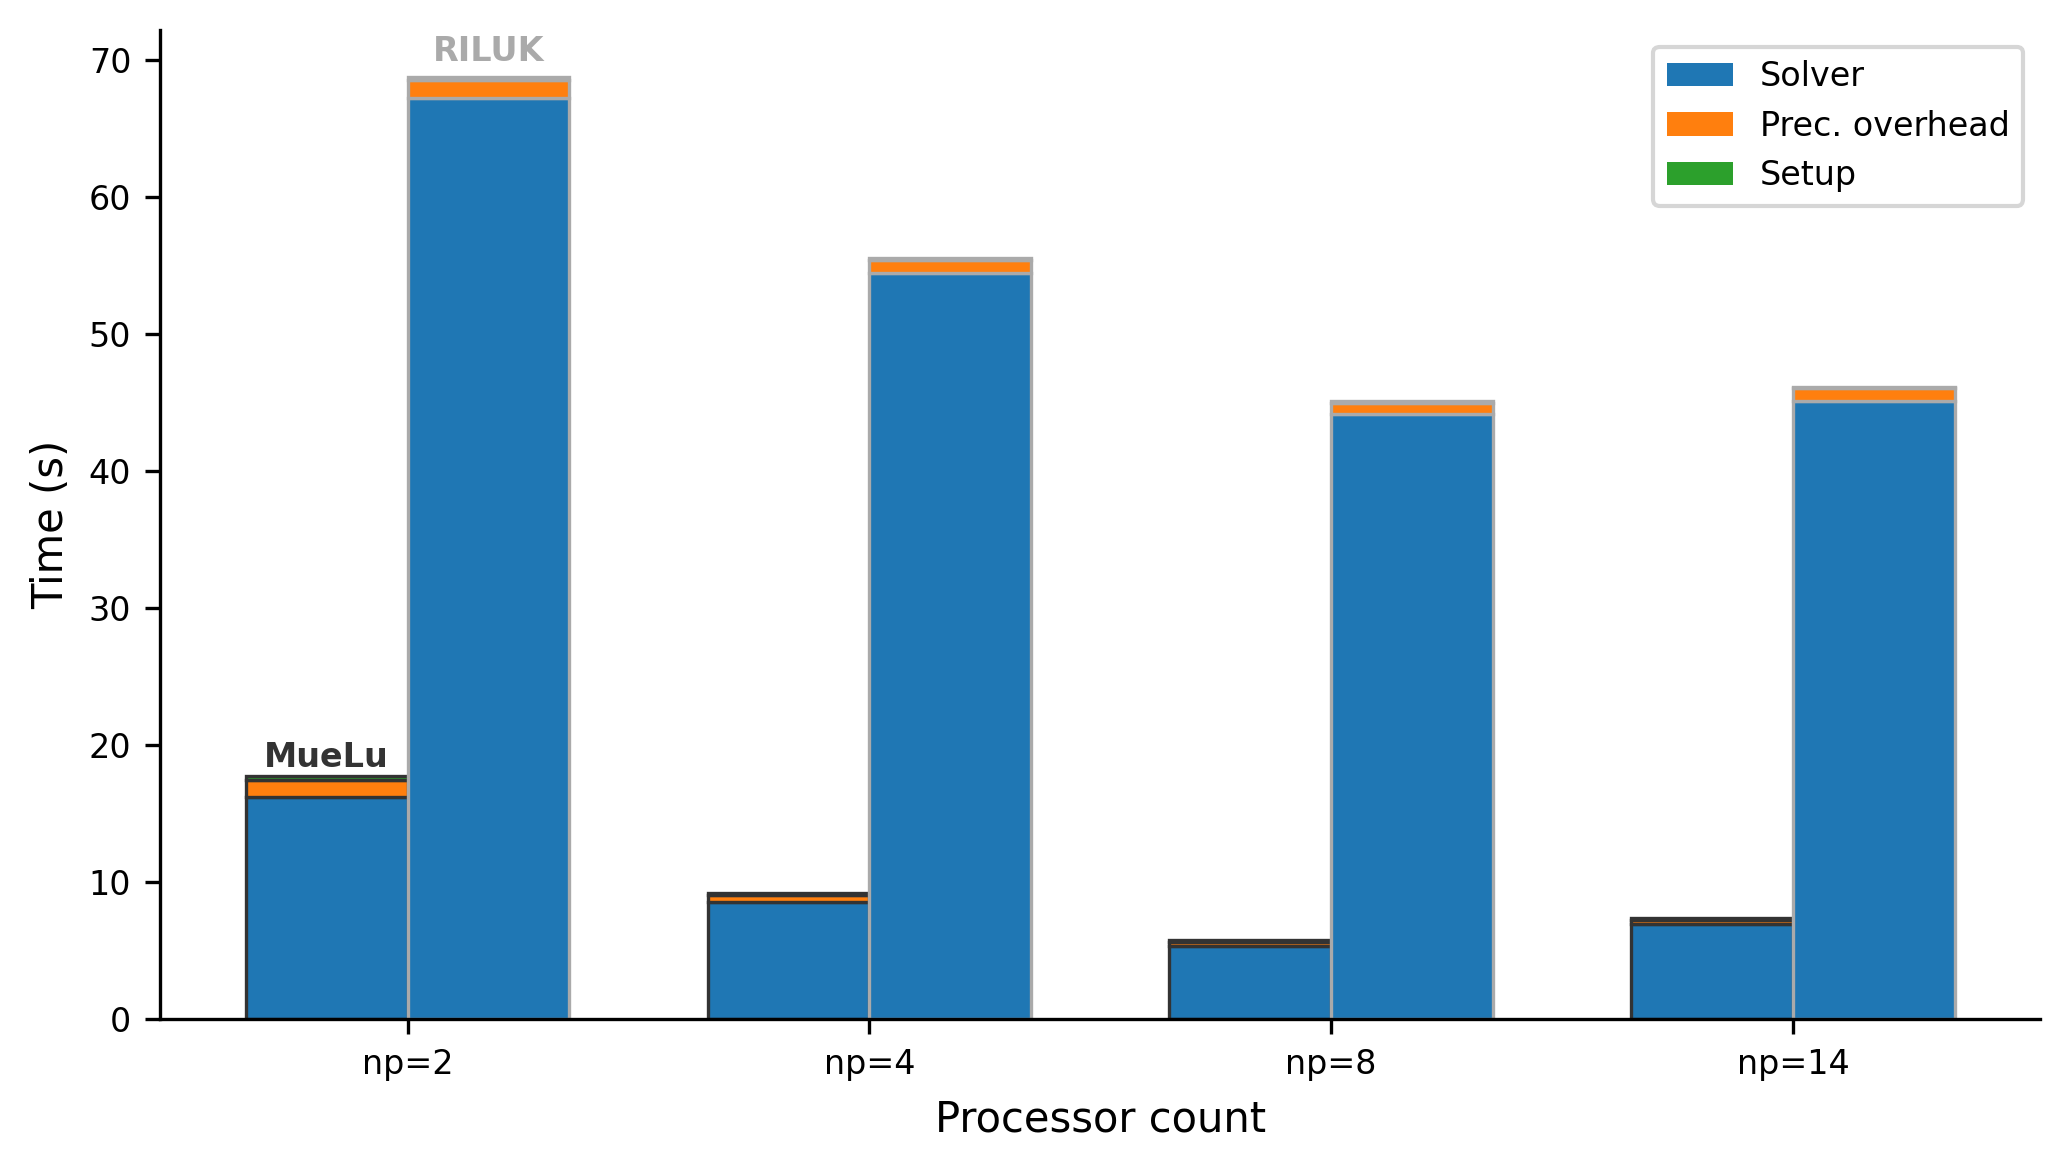
\includegraphics[width=0.9\textwidth]
	{../convergenceAnalysis/plotsAndData/optimalRun/time_breakdown.png}
	\caption{Time breakdown by section of the application. Setup involves reading the $\jR$ source and computing the conductivities. Preconditioner overhead displays the difference between the reported solve time by Belos and the wall clock time of the entire solve procedure. Solver is the reported solve time from Belos.}
	\label{fig:time_breakdown}
\end{figure}
\subsubsection{Summary}
While not a comprehensive analysis of the performance of this application, this study was used as a starting point to determine solver and preconditioner parameters. This provided a performance baseline that can be used to build and test the application. However, a more comprehensive study of solver runtime improvements is planned to be performed once the MHD interpolation is complete. The best performing MueLu-preconditioned GMRES configuration is used for all potential solves presented in Chapter~\ref{chap:results}.

\chapter{Results}
\label{chap:results}

This chapter presents solutions to the ionosphere surface equation (Equation~\ref{eqn:continuity_eqn}) over seasonal and geomagnetic variation. All solves use the MueLu-preconditioned GMRES solver that was discussed in Section~\ref{sec:convergence_analysis}. Since the magnetosphere-ionosphere coupling is still in progress, these plots present the results of a single southward IMF source term that was provided by the magnetosphere model and interpolation used in~\citet{global_groth_2000}. Figure~\ref{fig:sourceTerm} shows the source term that was used in this analysis.
\begin{figure}[htbp]
	\centering
	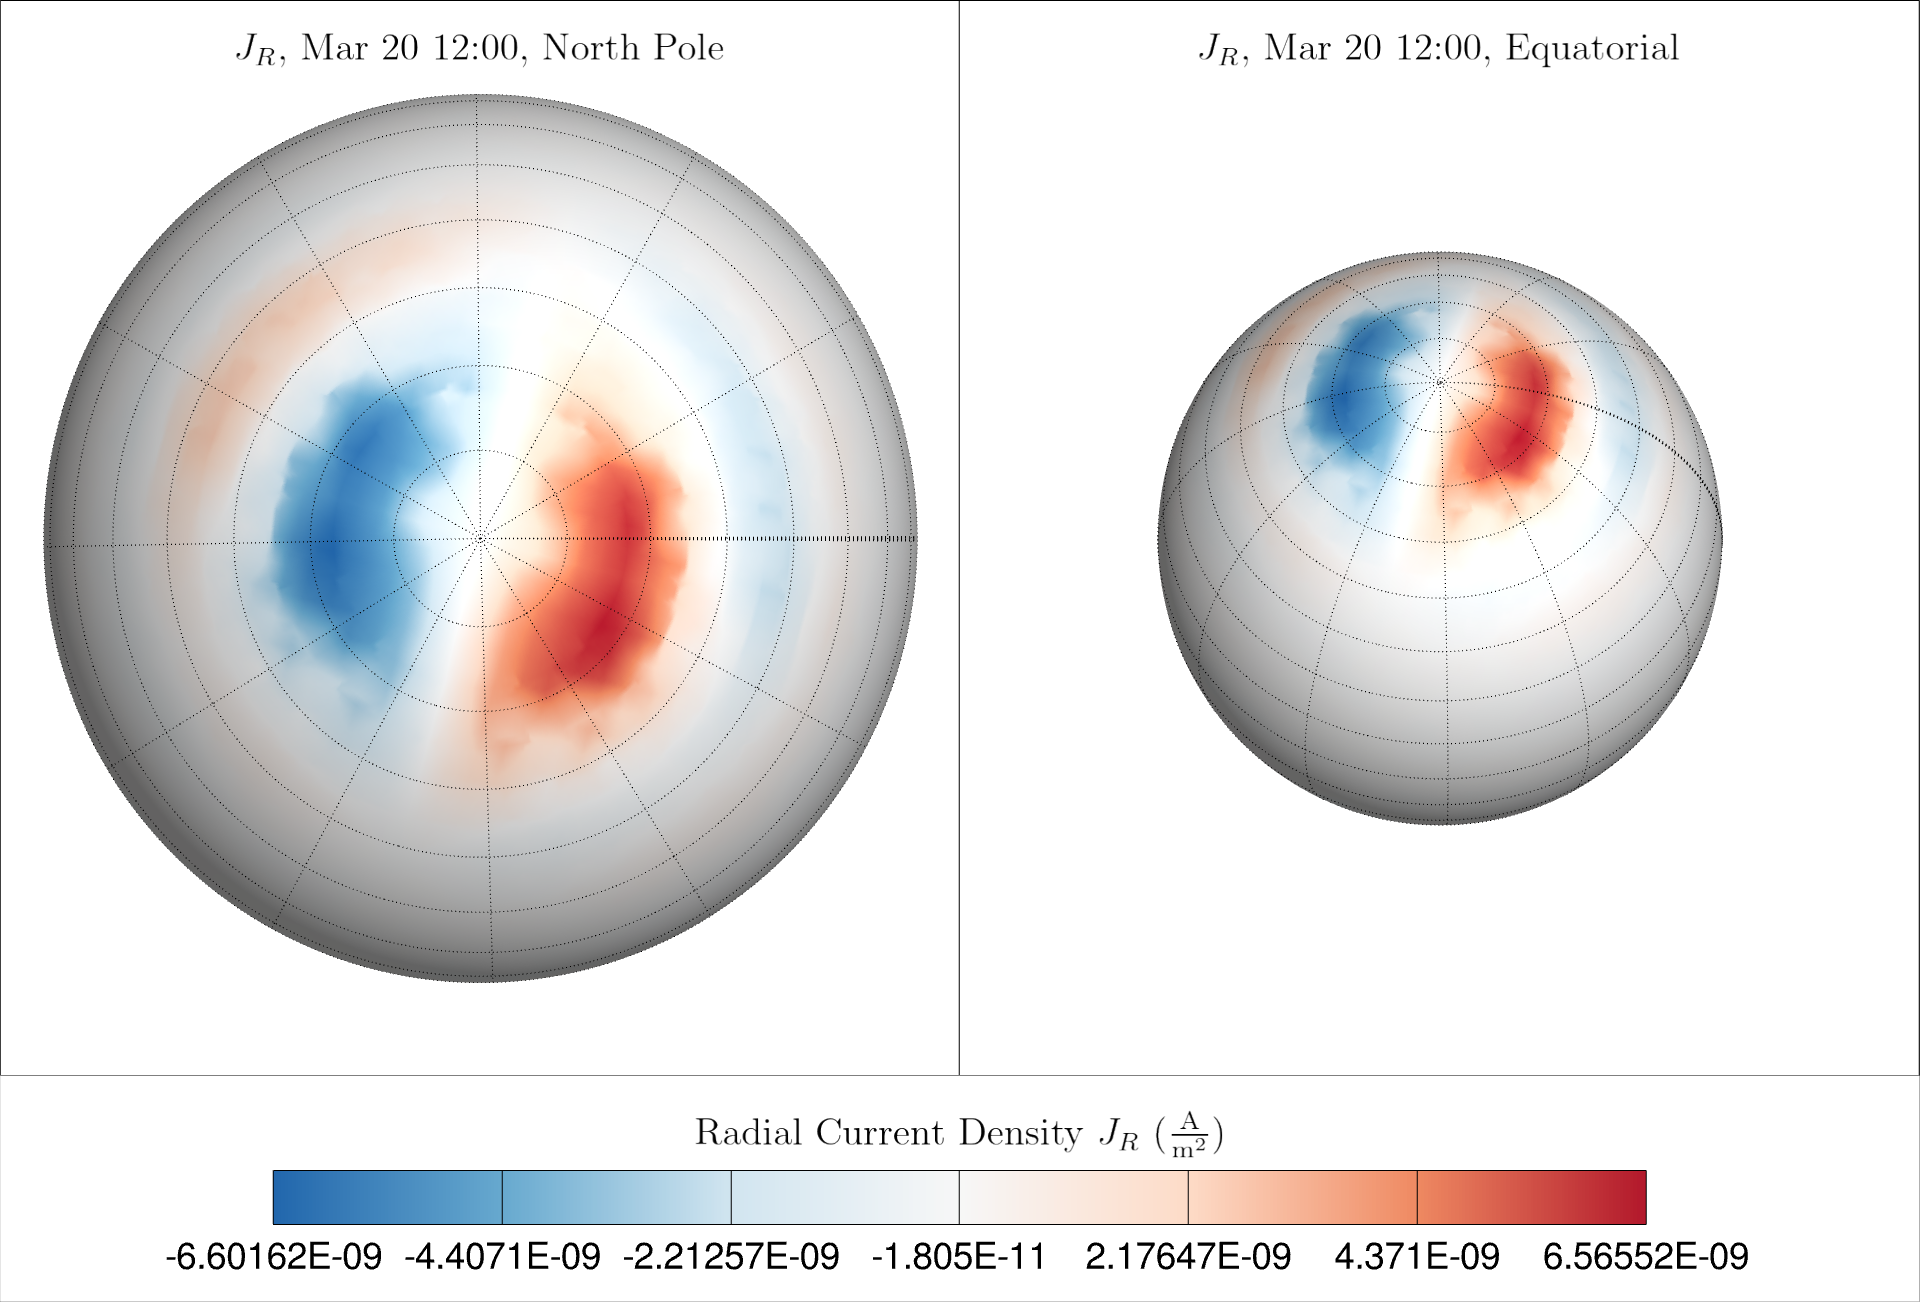
\includegraphics[width=0.67\textwidth]{figures/soureTerm.png}
	\caption{Radial current density $J_R$ ($\mathrm{A/m^2}$) at equinox (Mar 20, 12:00), showing the field-aligned current source term that drives the ionospheric electric potentials.}
	\label{fig:sourceTerm}
\end{figure}

\section{Geomagnetic Variation}
The $K_p$ index is a standardized index used to monitor geomagnetic disturbances on a global scale. It is calculated as the mean of observations from 13 contributing sub-auroral geomagnetic observatories. This is used to categorize the magnitude of geomagnetic disturbance and its irregularity into a quasi-logarithmic scale~\citep{matzka}. Figure~\ref{fig:potentialVsKp} shows the effect of increasing $K_p$ indices on the potential distribution of the ionosphere.
\begin{figure}[htbp]
	\centering
	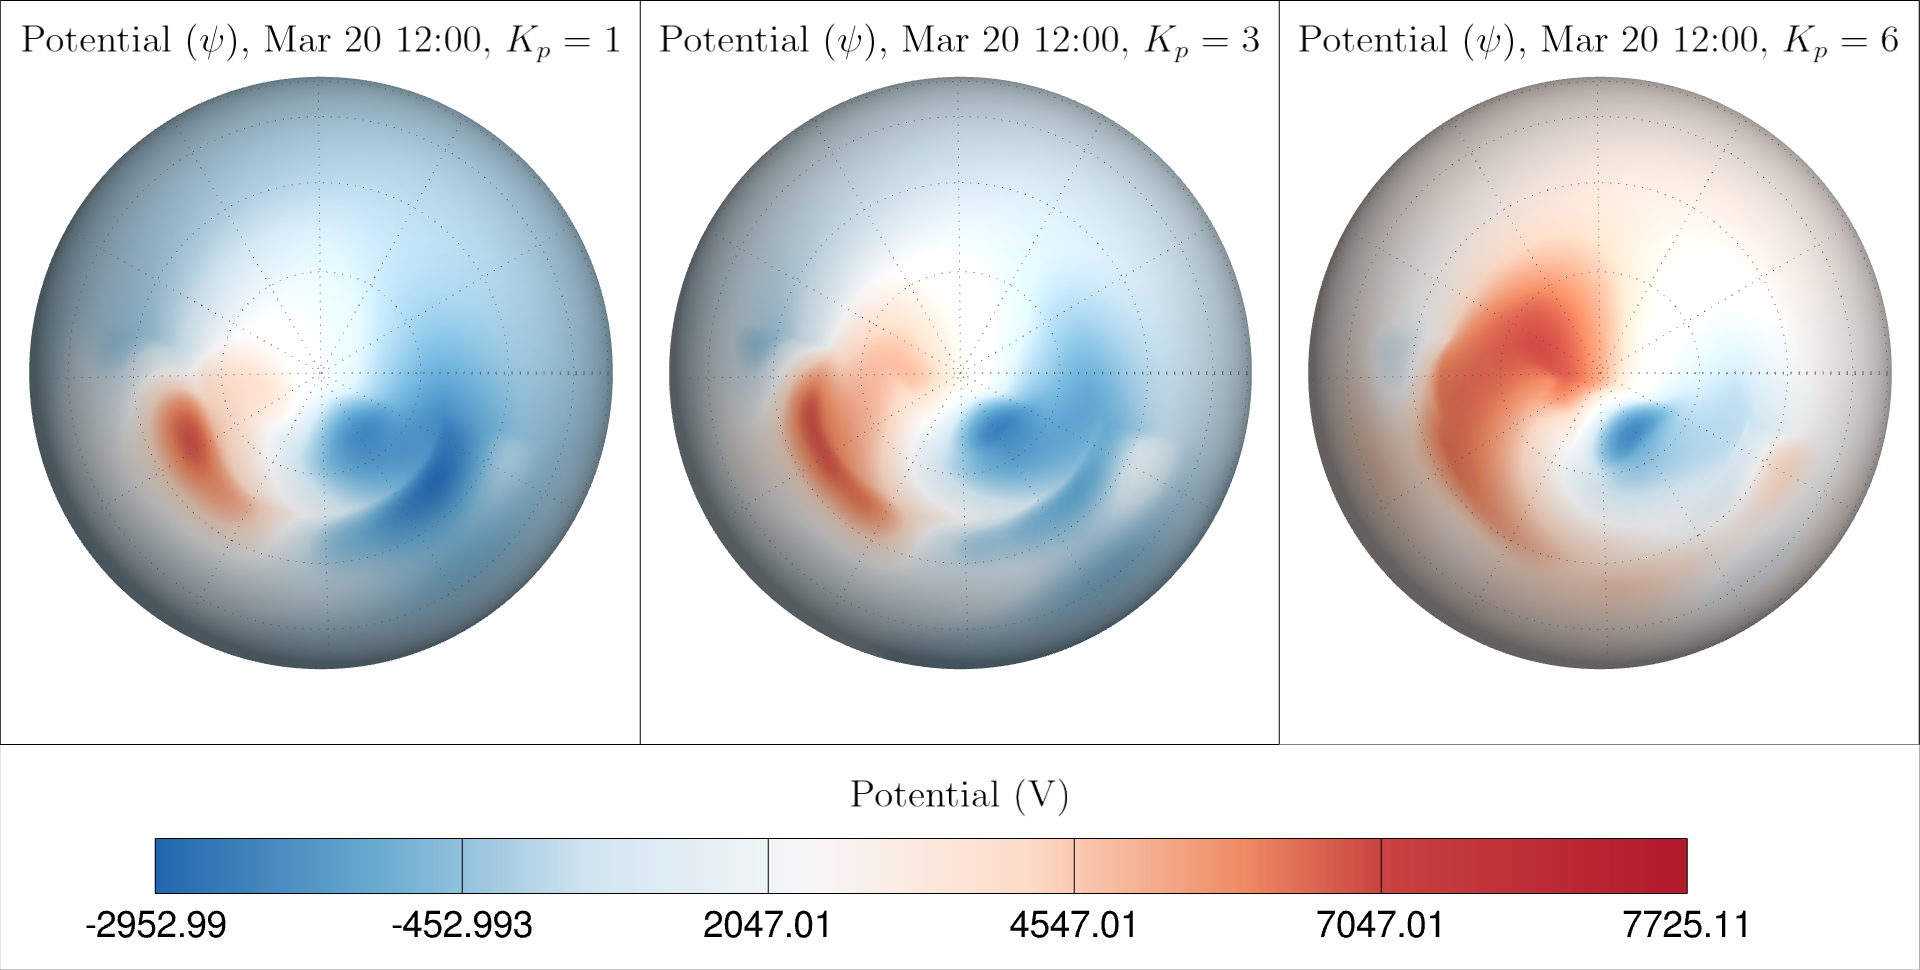
\includegraphics[width=\textwidth]{figures/potentialVsKp.png}
	\caption{Electric potential $\psi$ at the North Pole for $K_p = 1$, $3$, and $6$ at equinox (Mar 20, 12:00), showing the increasing size of the convection cells.}
	\label{fig:potentialVsKp}
\end{figure}
As shown in Figure~\ref{fig:auroralPedersonVsKp}, higher $K_p$ values generally correspond with a larger region affected by auroral precipitation. Figure~\ref{fig:potentialVsKp} shows the resulting two-cell pattern that is consistent with a southward IMF~\citep{kelley2009}. The higher $K_p$ values show a much more spread out structure for the convection cells. Conversely, in the low $K_p$ case the cells cover a significantly smaller region. During periods of high geomagnetic activity, this will result in the ionospheric currents affecting infrastructure at lower latitudes.
\section{Seasonal Variation}
\begin{figure}[H]
	\centering
	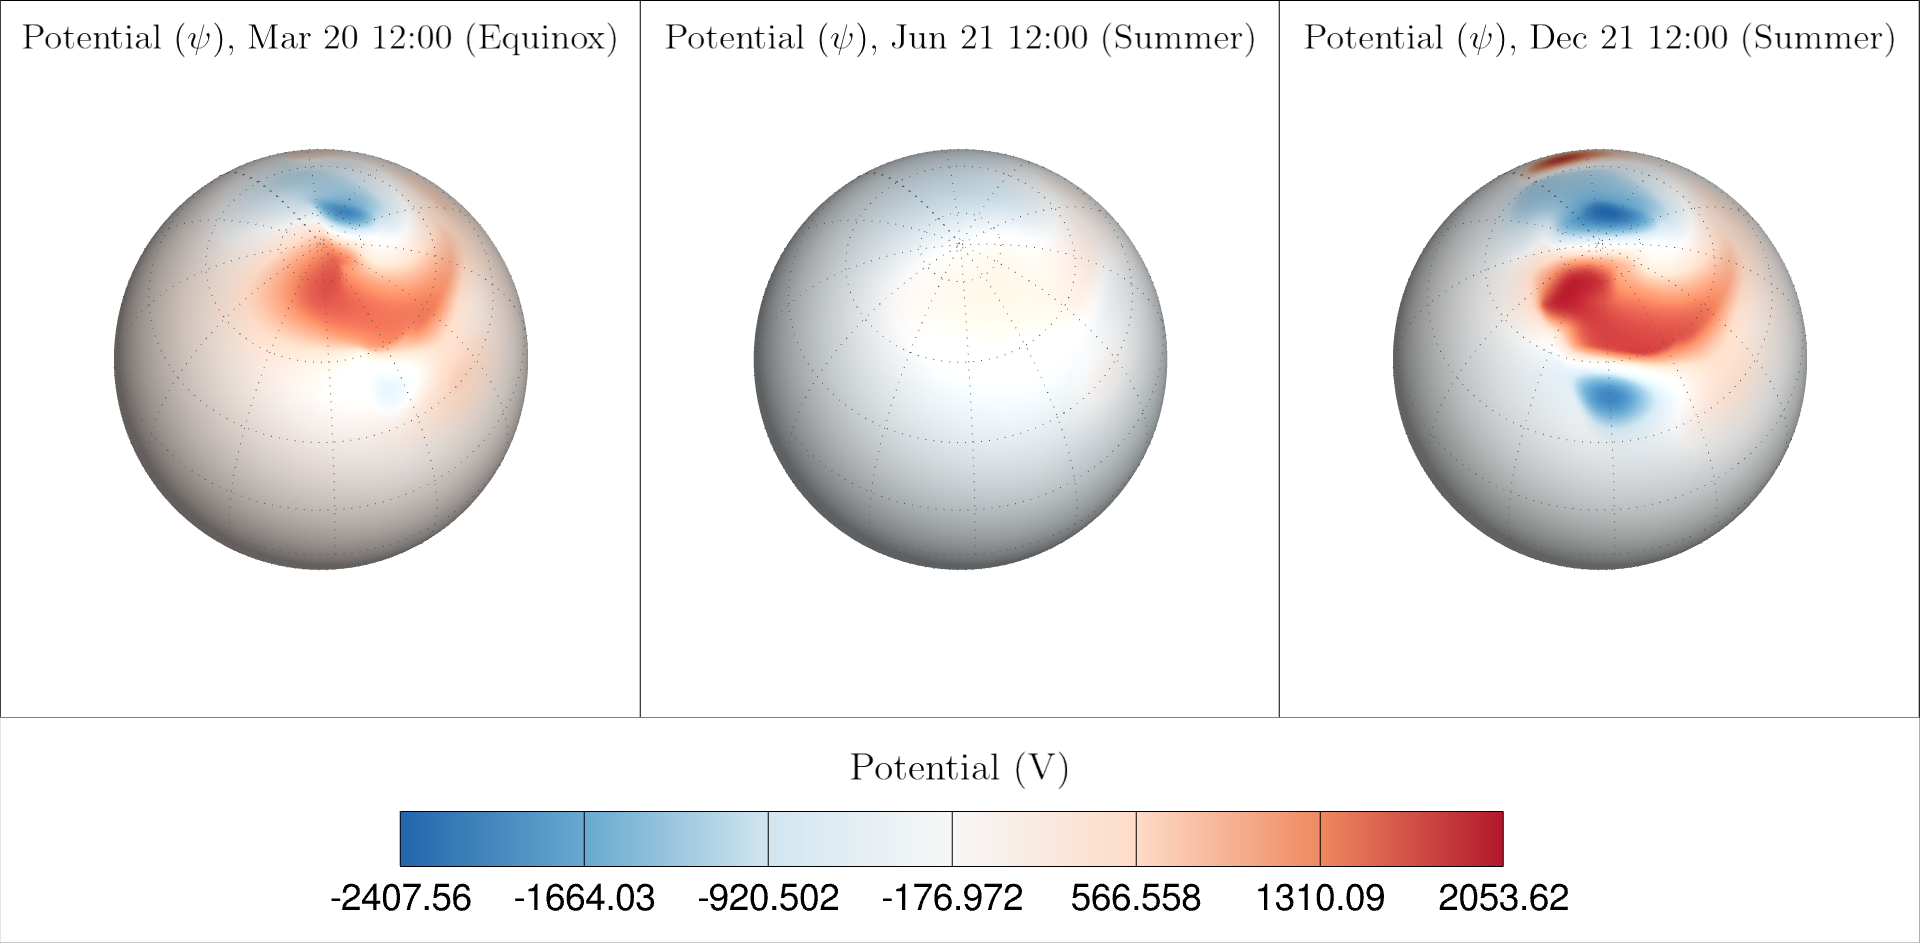
\includegraphics[width=\textwidth]{figures/potentialVsSeason.png}
	\caption{Electric potential $\psi$ at the North Pole for equinox (Mar 20), summer (Jun 21), and winter (Dec 21) at 12:00 UT, showing the seasonal effect on the intensity of the convection cells.}
	\label{fig:potentialVsSeason}
\end{figure}
Through the seasonal dependence of the conductivity discussed in Section~\ref{sec:euv_conductivity}, it is possible to analyse the behaviour of the potential solution over differing seasons. Figure~\ref{fig:potentialVsSeason} displays the seasonal variation of the potential for a spring equinox, northern-summer and northern-winter date. The varying conductivity due to sun inclination has a major effect on the intensity of the ionospheric convection cells.
\begin{figure}[H]
	\centering
	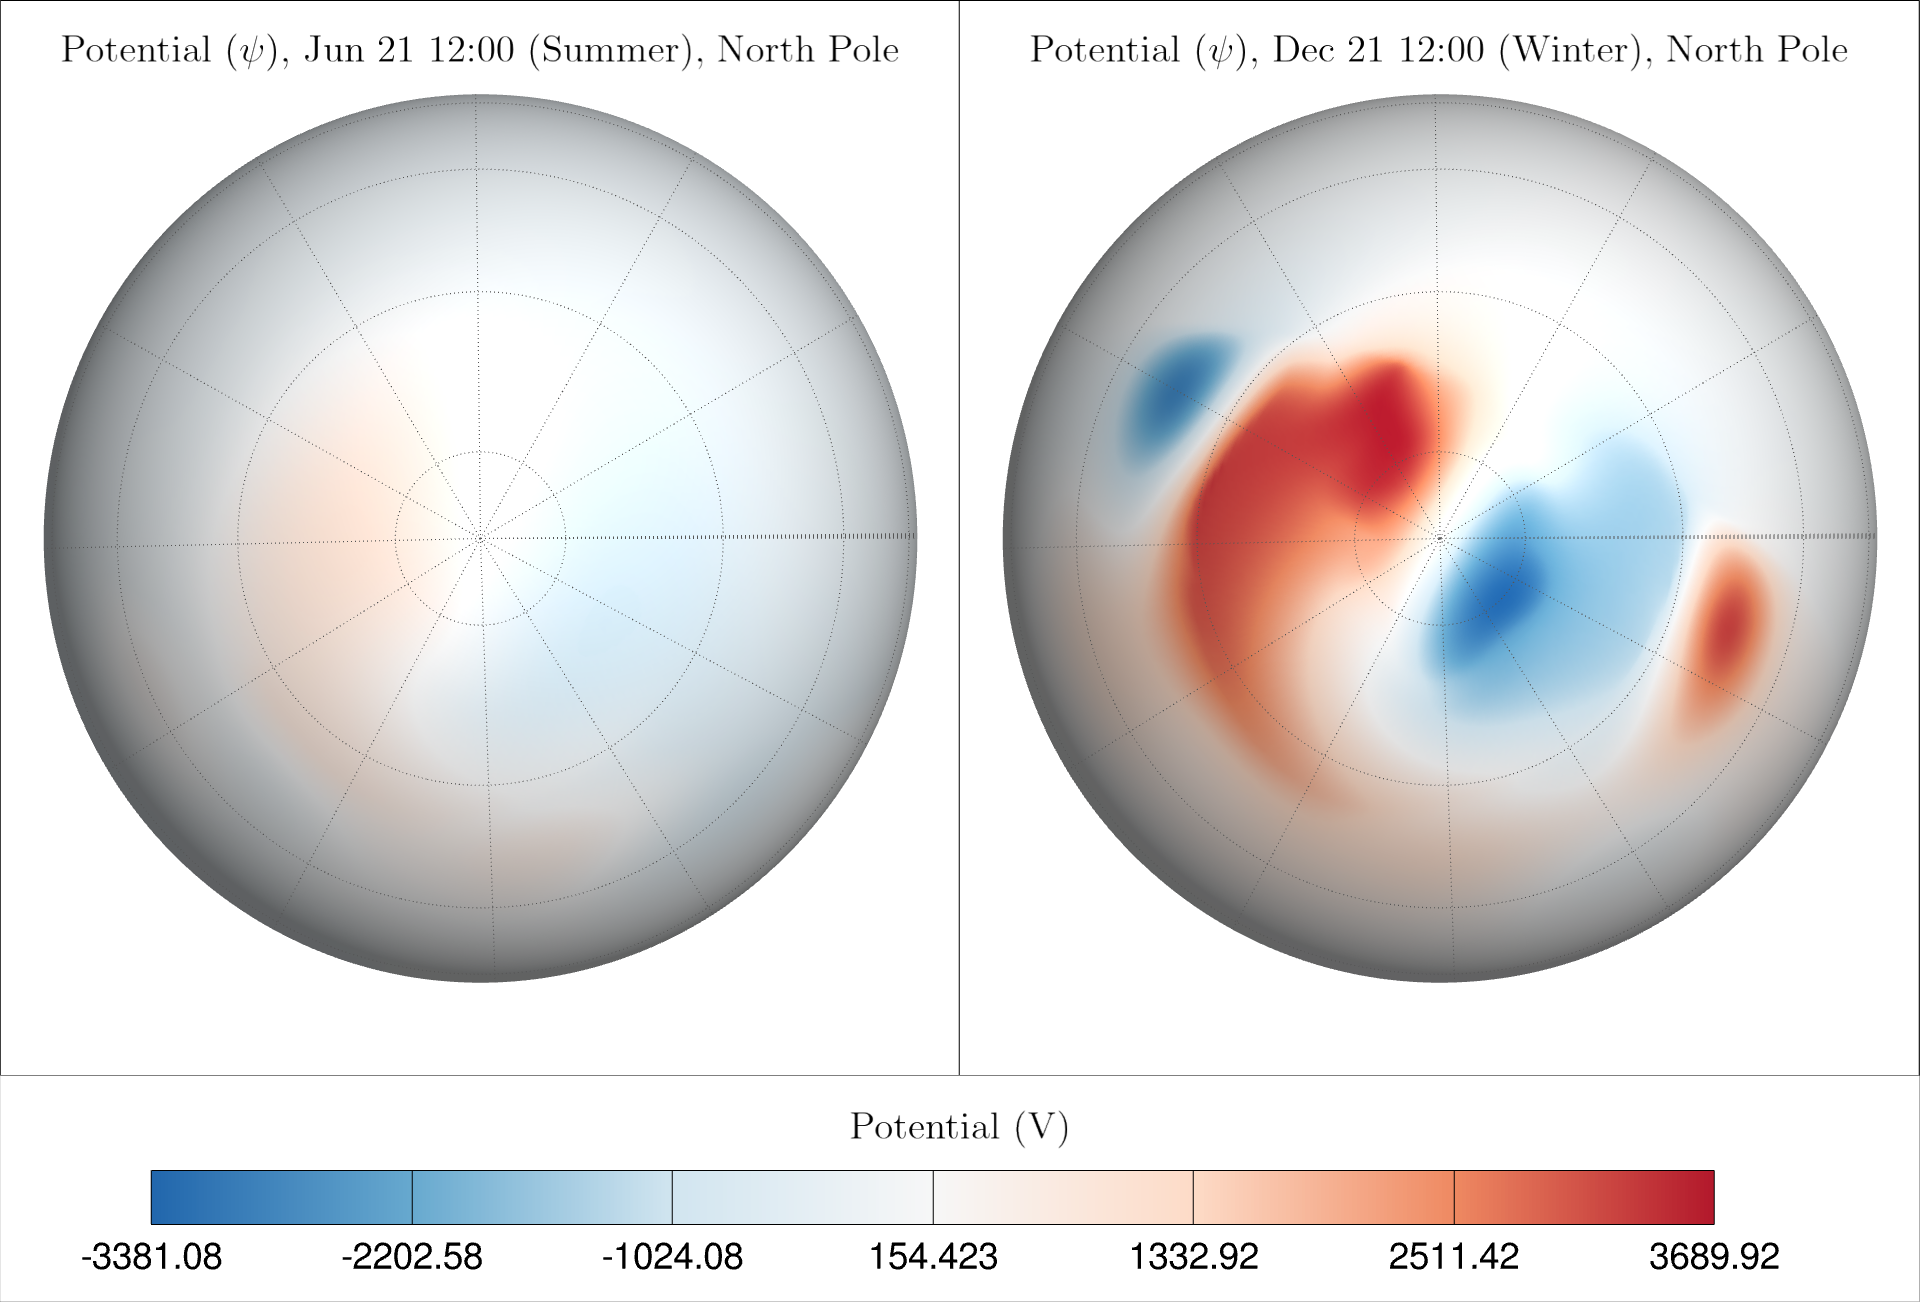
\includegraphics[width=.67\textwidth]{figures/potentialVsSeasonPole.png}
	\caption{Electric potential $\psi$ at the North Pole for summer (Jun 21), and winter (Dec 21) at 12:00 UT, showing the seasonal effect on the intensity of the convection cells.}
	\label{fig:potentialVsSeasonPole}
\end{figure}
Figure~\ref{fig:potentialVsSeasonPole} provides a clear display of the large differences that appear seasonally as viewed from above the north pole. As shown in Figure~\ref{fig:euvPedersonVsSeason}, the summer months represent a significantly higher level of conductance due to EUV ionization in the north pole. Due to this, the currents do not dissipate as much energy through the north pole convection cells. These results show that winter months can result in higher potential gradients in high latitude regions, increasing the probability of adverse interference with ground based infrastructure.
\begin{figure}[H]
	\centering
	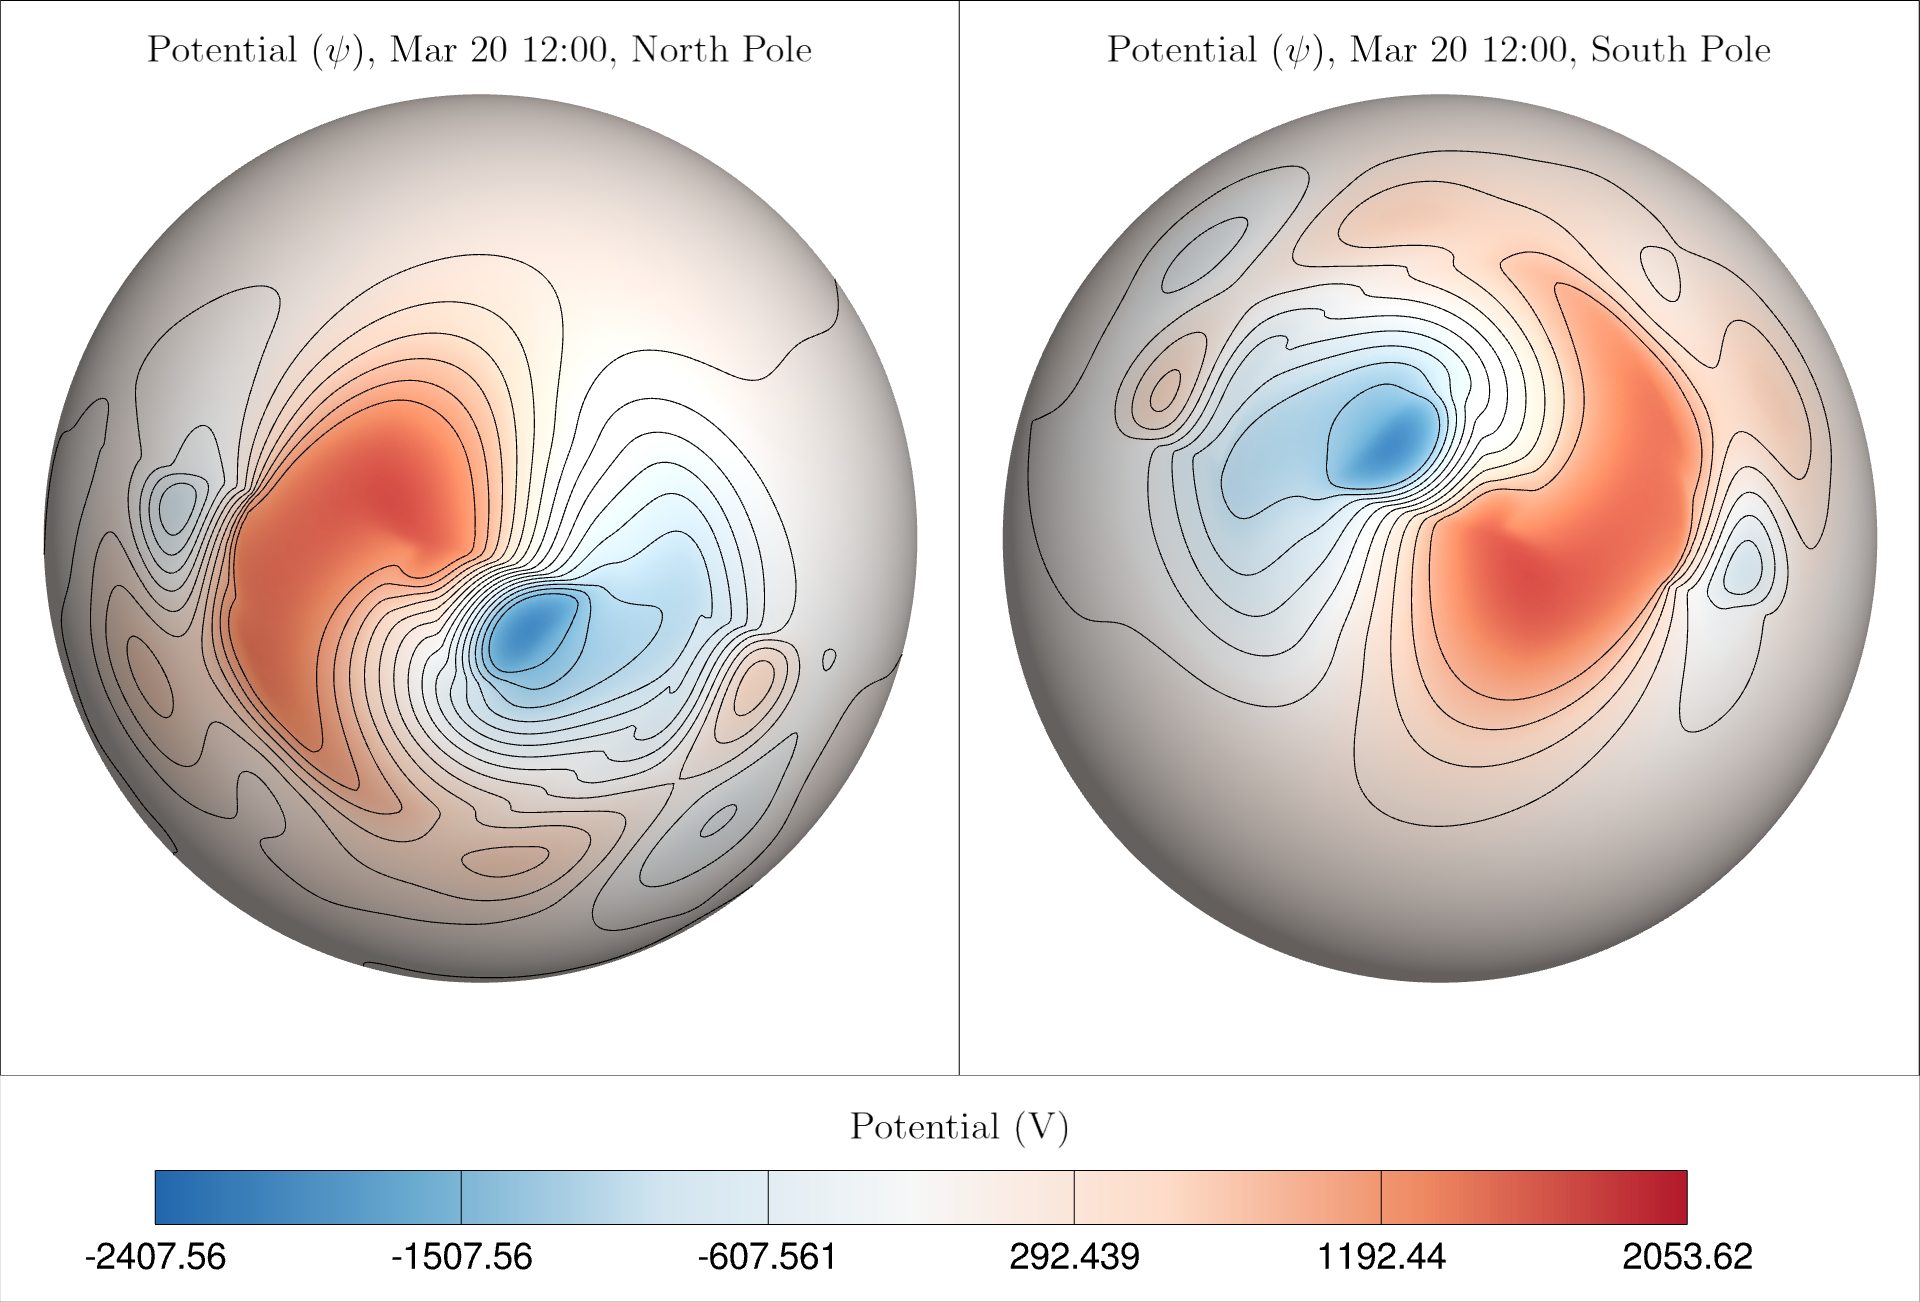
\includegraphics[width=\textwidth]{figures/poleContours.png}
	\caption{Electric potential $\psi$ at the north and south pole for equinox (Mar 20) conditions. Contour lines overlaid to show the continuity of the boundary condition.}
	\label{fig:boundaryCondition}
\end{figure}
These results exhibit clear continuous boundary behaviour at the poles (Figure~\ref{fig:boundaryCondition}) while showing a clear two-cell pattern that is characteristic of a southward IMF~\citep{kelley2009}. This qualitative analysis shows that the model obeys behaviour consistent with the known behaviour of the ionosphere. More robust verification of the model's predictions will become possible with the completion of the magnetosphere-ionosphere coupling procedure, allowing for a comprehensive study of varied radial current data.

\chapter{Conclusions and Future Work}
\section{Conclusion}
In this thesis a modular ionospheric model was presented to provide coupling to a global magnetohydrodynamic model of the magnetosphere. Empirical models were implemented for the ionospheric conductivity with future opportunity to provide multiple new models. Additionally, a spherical discretization of the ionospheric surface equation was provided with a physically grounded boundary condition. The application shown provides an extensible framework for ionosphere simulation with the ability to provide output across different conductivity models, equations and boundary conditions. Through the solver and preconditioner parameter sweep, substantial performance improvements in the runtime of the application were obtained, reducing solve time from approximately 140 seconds to 10.

The qualitative analysis of the simulation output provided verification of the general structure of the produced potentials and the boundary condition behaviour. While there is still work remaining on certain portions of the application such as the magnetosphere-ionosphere coupling process, the model acts as a proof of concept for an extensible ionosphere simulation. Through additional verification and optimization as detailed in the next section, this model will provide the dissipative boundary condition that will allow for accurate space weather simulation.
\section{Future Work}
\subsection{Magnetosphere-Ionosphere Coupling}
Magnetosphere-ionosphere coupling is the immediate priority for future work, enabling this model to be used for practical space-weather prediction purposes. The incompleteness of the magnetosphere-ionosphere coupling has limited the analysis that is possible to perform on the output of the model. Once the solver loop described in Section~\ref{sec:application_structure} can be closed by providing time-stepped radial current data from the simulation, new strategies can be investigated to provide potentially increased solver performance. Additionally, this will allow for validation of the model's correctness over a range of IMF source terms.
\subsection{Verification}
A comprehensive verification of the predictions of the model is planned once the magnetosphere-ionosphere coupling is complete. This will involve testing the model over a wide range of IMF source terms and validating its output against reference potentials. Possible targets for validation include techniques such as the AMIE procedure~\citep{richmond1988amie} and LOMPE~\citep{local_laundal_2022}, which provide procedures to map high-latitude electric fields from sets of localized observational data, and electrostatic potential distributions produced by the SuperDARN network through the approach described in~\citet{ruohoniemi1998superdarn}.

A more in-depth analysis of the correctness of the results produced by this model's boundary condition is another priority. The polar boundary condition provided qualitatively good results. However, additional validation of the potentials produced by this boundary condition is still planned. This will likely involve testing the boundary condition against a series of manufactured solutions to verify its correctness.

\subsection{Solver and Performance Extensions}
The analysis in Section~\ref{sec:convergence_study} of this report provided substantial gains in performance. Iteration count was reduced from approximately 1500 to 100, with an improvement in solve time from approximately 140 to 10 seconds. However, the goal for the final model is to achieve sub-second solve times under most conditions. To achieve this, a more in-depth study of the convergence behaviour of the simulation is required. This would include finer parameter tuning, testing on a more realistic system with dedicated cores or a networked MPI cluster and a broader study of different solvers and preconditioning methods.

Avenues to be explored are optimized MPI rank data distribution including testing interleaved row storage methods and using the Trilinos package Zoltan to automatically partition data. Additionally, experimenting with the \texttt{GCRO-DR} GMRES solver that recycles Krylov subspace information across solves is planned. The last optimization is particularly promising as it is designed for systems where the matrix structure is constant with sequentially changing source vectors. Depending on the time scale required by the implementation, it could be used to recycle data between solves potentially further improving performance~\citep{parks2006}.
\subsection{Model Extensions}
One of the primary design choices in this application was the extensibility provided by the application structure. In order to leverage this, future plans include additional empirical models for the conductivity, implementing a new conductivity tensor and a new boundary condition. Alternate empirical models for the Hall and Pedersen conductivities are available as shown in~\citet{cousins2015} and~\citet{local_laundal_2022}. Additionally, the implementation of a plasma-parameter approach utilizing the NRLMSIS~\citep{nrlmsis_emmert_2020} and IRI~\citep{international_bilitza_2022} models in conjunction with the equations described in Equation~\ref{eq:physical_conduct} is planned. This would provide an alternative source for conductivity data while also providing values for the parallel conductivity. The alternative conductivity tensor proposed by~\citet{goodman1995} is also planned to be implemented as this would remove the requirement for the parallel conductivity entirely, and would allow the comparison of the two conductivity tensors. An alternative boundary condition, that is in the process of implementation, utilizing a five-point stencil mapped onto a ring of ghost points around the pole is also going to be added to the model. This is likely to result in better convergence behaviour than the divergence theorem approach, but does not provide continuity over the pole as a constraint. Together these planned extensions demonstrate how the modular structure of the application allows for exploration of multiple physical models without changes to the solver.



\appendix
\chapter{Numerical Implementation}

\section{Convergence Analysis}
% ── RILUK Summary (side by side) ──────────────────────────────
\begin{table}[H]
	\tiny
  \begin{minipage}{0.48\textwidth}
	\centering
	\begin{tabular}{cccccc}
		\toprule
		\textbf{Fill} & \textbf{$\bm {n_{\rm blocks}}$} & \textbf{$\bm {\bm{n_{\rm procs}}}$} & \textbf{Convgd.} & \textbf{Iter} & \textbf{Time (s)} \\
		\midrule
		2             & 100                             & 2                              & False            & 1500          & 151.8             \\
		2             & 100                             & 4                              & False            & 1500          & 77.8              \\
		2             & 100                             & 8                              & False            & 1500          & 43.08             \\
		2             & 100                             & 14                             & False            & 1500          & 47.75             \\
		2             & 200                             & 2                              & False            & 1500          & 268.7             \\
		2             & 200                             & 4                              & False            & 1500          & 137.2             \\
		2             & 200                             & 8                              & False            & 1500          & 76.38             \\
		2             & 200                             & 14                             & False            & 1500          & 84.09             \\
		2             & 500                             & 2                              & True             & 941           & 389               \\
		2             & 500                             & 4                              & True             & 979           & 213.3             \\
		2             & 500                             & 8                              & True             & 1256          & 142.4             \\
		2             & 500                             & 14                             & True             & 1422          & 183.4             \\
		\midrule
		5             & 100                             & 2                              & False            & 1500          & 154.8             \\
		5             & 100                             & 4                              & False            & 1500          & 79.17             \\
		5             & 100                             & 8                              & False            & 1500          & 44.16             \\
		5             & 100                             & 14                             & False            & 1500          & 48.88             \\
		5             & 200                             & 2                              & True             & 507           & 86.18             \\
		5             & 200                             & 4                              & True             & 784           & 73.32             \\
		5             & 200                             & 8                              & False            & 1500          & 77.55             \\
		5             & 200                             & 14                             & False            & 1500          & 85.13             \\
		5             & 500                             & 2                              & True             & 286           & 73.68             \\
		5             & 500                             & 4                              & True             & 331           & 49.7              \\
		5             & 500                             & 8                              & True             & 401           & 40.86             \\
		5             & 500                             & 14                             & True             & 491           & 65.46             \\
		\midrule
		10            & 100                             & 2                              & True             & 391           & 41.38             \\
		10            & 100                             & 4                              & True             & 697           & 38.54             \\
		10            & 100                             & 8                              & False            & 1500          & 47.8              \\
		10            & 100                             & 14                             & False            & 1500          & 51.64             \\
		10            & 200                             & 2                              & True             & 196           & 36.86             \\
		10            & 200                             & 4                              & True             & 355           & 31.99             \\
		\bottomrule
	\end{tabular}
	\captionof{table}{Rows 1--30}
  \end{minipage}
  \begin{minipage}{0.48\textwidth}
	\centering
	\begin{tabular}{cccccc}
		\toprule
		\textbf{Fill} & \textbf{$\bm {n_{\rm blocks}}$} & \textbf{$\bm{n_{\rm procs}}$} & \textbf{Convgd.} & \textbf{Iter} & \textbf{Time (s)} \\
		\midrule
		10            & 200                             & 8                        & True             & 554           & 29.43             \\
		10            & 200                             & 14                       & True             & 978           & 58.21             \\
		10            & 500                             & 2                        & True             & 196           & 36.82             \\
		10            & 500                             & 4                        & True             & 252           & 30.28             \\
		10            & 500                             & 8                        & True             & 313           & 26.24             \\
		10            & 500                             & 14                       & True             & 402           & 45.26             \\
		\midrule
		15            & 100                             & 2                        & False            & --            & --                \\
		15            & 100                             & 4                        & False            & --            & --                \\
		15            & 100                             & 8                        & False            & --            & --                \\
		15            & 100                             & 14                       & False            & --            & --                \\
		15            & 200                             & 2                        & False            & --            & --                \\
		15            & 200                             & 4                        & False            & --            & --                \\
		15            & 200                             & 8                        & False            & --            & --                \\
		15            & 200                             & 14                       & False            & --            & --                \\
		15            & 500                             & 2                        & False            & --            & --                \\
		15            & 500                             & 4                        & False            & --            & --                \\
		15            & 500                             & 8                        & False            & --            & --                \\
		15            & 500                             & 14                       & False            & --            & --                \\
		\midrule
		20            & 100                             & 2                        & False            & --            & --                \\
		20            & 100                             & 4                        & False            & --            & --                \\
		20            & 100                             & 8                        & False            & --            & --                \\
		20            & 100                             & 14                       & False            & --            & --                \\
		20            & 200                             & 2                        & False            & --            & --                \\
		20            & 200                             & 4                        & False            & --            & --                \\
		20            & 200                             & 8                        & False            & --            & --                \\
		20            & 200                             & 14                       & False            & --            & --                \\
		20            & 500                             & 2                        & False            & --            & --                \\
		20            & 500                             & 4                        & False            & --            & --                \\
		20            & 500                             & 8                        & False            & --            & --                \\
		20            & 500                             & 14                       & False            & --            & --                \\
		\bottomrule
	\end{tabular}
  \captionof{table}{Rows 31--60}
\end{minipage}
\caption{Raw results from the parameter sweep timing experiment in Section~\ref{sec:convergence_study} for the IfPack2 \texttt{RILUK} preconditioner. Displays preconditioner parameters that were tested, number of processors, convergence status, final iteration count and time as reported by the Belos solve time. Results are grouped by processor count.}
\label{tab:ifpack_results}
\end{table}
\newpage
% ── MueLu Summary ──────────────────────────────────────────────
\begin{table}[H]
	\centering
  \footnotesize
	\begin{tabular}{cccccc}
		\toprule
		\textbf{Fill} & \textbf{$\bm {n_{\rm blocks}}$} & \textbf{$\bm{n_{\rm procs}}$} & \textbf{Convgd.} & \textbf{Iter} & \textbf{Time (s)} \\
		\midrule
		1             & 100                             & 2                        & False            & 1500          & 159.3             \\
		1             & 100                             & 4                        & False            & 1500          & 84.39             \\
		1             & 100                             & 8                        & True             & 722           & 23.4              \\
		1             & 100                             & 14                       & False            & 1500          & 53.9              \\
		1             & 200                             & 2                        & False            & 576           & 106.5             \\
		1             & 200                             & 4                        & False            & 1500          & 144.6             \\
		1             & 200                             & 8                        & True             & 356           & 18.72             \\
		1             & 200                             & 14                       & True             & 581           & 35.09             \\
		1             & 500                             & 2                        & False            & 243           & 55.04             \\
		1             & 500                             & 4                        & False            & 760           & 146.8             \\
		1             & 500                             & 8                        & False            & 227           & 14.45             \\
		1             & 500                             & 14                       & True             & 277           & 22.49             \\
		\midrule
		2             & 100                             & 2                        & True             & 291           & 30.69             \\
		2             & 100                             & 4                        & True             & 583           & 32.65             \\
		2             & 100                             & 8                        & True             & 592           & 19.68             \\
		2             & 100                             & 14                       & False            & 1500          & 54.65             \\
		2             & 200                             & 2                        & True             & 151           & 22.68             \\
		2             & 200                             & 4                        & True             & 170           & 14.69             \\
		2             & 200                             & 8                        & True             & 183           & 9.88              \\
		2             & 200                             & 14                       & True             & 359           & 20.61             \\
		2             & 500                             & 2                        & True             & 151           & 22.7              \\
		2             & 500                             & 4                        & True             & 170           & 14.64             \\
		2             & 500                             & 8                        & True             & 183           & 9.824             \\
		2             & 500                             & 14                       & True             & 232           & 16.23             \\
		\midrule
		4             & 100                             & 2                        & True             & 89            & 9.054             \\
		4             & 100                             & 4                        & True             & 91            & 4.956             \\
		4             & 100                             & 8                        & True             & 98            & 3.327             \\
		4             & 100                             & 14                       & True             & 191           & 6.926             \\
		4             & 200                             & 2                        & True             & 89            & 9.07              \\
		4             & 200                             & 4                        & True             & 91            & 4.945             \\
		4             & 200                             & 8                        & True             & 98            & 3.345             \\
		4             & 200                             & 14                       & True             & 134           & 6.151             \\
		4             & 500                             & 2                        & True             & 89            & 9.075             \\
		4             & 500                             & 4                        & True             & 91            & 5.003             \\
		4             & 500                             & 8                        & True             & 98            & 3.339             \\
		4             & 500                             & 14                       & True             & 134           & 6.17              \\
		\bottomrule
	\end{tabular}
\caption{Raw results from the parameter sweep timing experiment in Section~\ref{sec:convergence_study} for the MueLu with \texttt{RILUK} smoother and coarse solver preconditioner. Displays preconditioner parameters that were tested, number of processors, convergence status, final iteration count and time as reported by the Belos solve time. Results are grouped by processor count.}
	\label{tab:muelu_results}
\end{table}

% ── Ifpack2 Optimal ────────────────────────────────────────────
\begin{table}[H]
  \scriptsize
	\centering
	\resizebox{\textwidth}{!}{%
		\begin{tabular}{cccccccc}
			\toprule
			\textbf{Fill} & \textbf{$\bm {n_{\rm blocks}}$} & \textbf{$\bm{n_{\rm procs}}$} & \textbf{Rep} & \textbf{Convgd.} & \textbf{Wall Time (s)} & \textbf{Iter} & \textbf{Time (s)} \\
			\midrule
			10            & 500                             & 2                        & 1            & True             & --                     & 196           & 68.08             \\
			10            & 500                             & 2                        & 2            & True             & 70.31                  & 196           & 67.07             \\
			10            & 500                             & 2                        & 3            & True             & 70.36                  & 196           & 67.11             \\
			10            & 500                             & 2                        & 4            & True             & 70.38                  & 196           & 67.14             \\
			10            & 500                             & 2                        & 5            & True             & 70.29                  & 196           & 67.03             \\
			10            & 500                             & 2                        & 6            & True             & 70.3                   & 196           & 67.05             \\
			10            & 500                             & 2                        & 7            & True             & 70.31                  & 196           & 67.05             \\
			10            & 500                             & 2                        & 8            & True             & 70.34                  & 196           & 67.1              \\
			10            & 500                             & 2                        & 9            & True             & 70.34                  & 196           & 67.09             \\
			10            & 500                             & 2                        & 10           & True             & 70.45                  & 196           & 67.2              \\
			\midrule
			10            & 500                             & 4                        & 1            & True             & 57.3                   & 252           & 54.4              \\
			10            & 500                             & 4                        & 2            & True             & 57.23                  & 252           & 54.34             \\
			10            & 500                             & 4                        & 3            & True             & 57.29                  & 252           & 54.4              \\
			10            & 500                             & 4                        & 4            & True             & 57.51                  & 252           & 54.62             \\
			10            & 500                             & 4                        & 5            & True             & 57.33                  & 252           & 54.44             \\
			10            & 500                             & 4                        & 6            & True             & 57.42                  & 252           & 54.53             \\
			10            & 500                             & 4                        & 7            & True             & 57.45                  & 252           & 54.56             \\
			10            & 500                             & 4                        & 8            & True             & 57.36                  & 252           & 54.47             \\
			10            & 500                             & 4                        & 9            & True             & 57.32                  & 252           & 54.42             \\
			10            & 500                             & 4                        & 10           & True             & 57.45                  & 252           & 54.58             \\
			\midrule
			10            & 500                             & 8                        & 1            & True             & 46.82                  & 313           & 44.06             \\
			10            & 500                             & 8                        & 2            & True             & 46.92                  & 313           & 44.17             \\
			10            & 500                             & 8                        & 3            & True             & 46.94                  & 313           & 44.18             \\
			10            & 500                             & 8                        & 4            & True             & 46.97                  & 313           & 44.2              \\
			10            & 500                             & 8                        & 5            & True             & 46.95                  & 313           & 44.17             \\
			10            & 500                             & 8                        & 6            & True             & 46.96                  & 313           & 44.21             \\
			10            & 500                             & 8                        & 7            & True             & 46.96                  & 313           & 44.2              \\
			10            & 500                             & 8                        & 8            & True             & 46.99                  & 313           & 44.24             \\
			10            & 500                             & 8                        & 9            & True             & 46.95                  & 313           & 44.19             \\
			10            & 500                             & 8                        & 10           & True             & 46.93                  & 313           & 44.17             \\
			\midrule
			10            & 500                             & 14                       & 1            & True             & 48.03                  & 402           & 45.15             \\
			10            & 500                             & 14                       & 2            & True             & 47.99                  & 402           & 45.12             \\
			10            & 500                             & 14                       & 3            & True             & 48.04                  & 402           & 45.16             \\
			10            & 500                             & 14                       & 4            & True             & 47.99                  & 402           & 45.12             \\
			10            & 500                             & 14                       & 5            & True             & 47.97                  & 402           & 45.08             \\
			10            & 500                             & 14                       & 6            & True             & 47.96                  & 402           & 45.1              \\
			10            & 500                             & 14                       & 7            & True             & 47.98                  & 402           & 45.09             \\
			10            & 500                             & 14                       & 8            & True             & 47.96                  & 402           & 45.08             \\
			10            & 500                             & 14                       & 9            & True             & 48.07                  & 402           & 45.2              \\
			10            & 500                             & 14                       & 10           & True             & 47.97                  & 402           & 45.09             \\
			\bottomrule
		\end{tabular}
	}% end resizebox
	\caption{Ifpack2 RILUK best performing configuration results. Displays preconditioner parameters that were tested, number of processors, convergence status, final iteration count and time as reported by the Belos solve time. Wall clock time indicates the total runtime of the solve step including startup. Results are grouped by processor count.}
	\label{tab:ifpack_optimal}

\end{table}



% ── MueLu Optimal ──────────────────────────────────────────────
\begin{table}[H]
	\centering
	\scriptsize
	\resizebox{\textwidth}{!}{%
		\begin{tabular}{cccccccc}
			\toprule
			\textbf{Fill} & \textbf{$\bm {n_{\rm blocks}}$} & \textbf{$\bm{n_{\rm procs}}$} & \textbf{Rep} & \textbf{Convgd.} & \textbf{Wall Time (s)} & \textbf{Iter} & \textbf{Time (s)} \\
			\midrule
			4             & 100                             & 2                            & 1            & True             & --                     & 89            & 16.33             \\
			4             & 100                             & 2                            & 2            & True             & 19.25                  & 89            & 16.18             \\
			4             & 100                             & 2                            & 3            & True             & 19.26                  & 89            & 16.2              \\
			4             & 100                             & 2                            & 4            & True             & 19.28                  & 89            & 16.22             \\
			4             & 100                             & 2                            & 5            & True             & 19.28                  & 89            & 16.21             \\
			4             & 100                             & 2                            & 6            & True             & 19.29                  & 89            & 16.21             \\
			4             & 100                             & 2                            & 7            & True             & 19.29                  & 89            & 16.22             \\
			4             & 100                             & 2                            & 8            & True             & 19.24                  & 89            & 16.17             \\
			4             & 100                             & 2                            & 9            & True             & 19.31                  & 89            & 16.24             \\
			4             & 100                             & 2                            & 10           & True             & 19.29                  & 89            & 16.21             \\
			\midrule
			4             & 100                             & 4                            & 1            & True             & 11.01                  & 91            & 8.521             \\
			4             & 100                             & 4                            & 2            & True             & 11.02                  & 91            & 8.54              \\
			4             & 100                             & 4                            & 3            & True             & 11.03                  & 91            & 8.528             \\
			4             & 100                             & 4                            & 4            & True             & 11.01                  & 91            & 8.53              \\
			4             & 100                             & 4                            & 5            & True             & 11.01                  & 91            & 8.521             \\
			4             & 100                             & 4                            & 6            & True             & 11.02                  & 91            & 8.528             \\
			4             & 100                             & 4                            & 7            & True             & 11.03                  & 91            & 8.527             \\
			4             & 100                             & 4                            & 8            & True             & 11.01                  & 91            & 8.535             \\
			4             & 100                             & 4                            & 9            & True             & 11.01                  & 91            & 8.517             \\
			4             & 100                             & 4                            & 10           & True             & 11.04                  & 91            & 8.552             \\
			\midrule
			4             & 100                             & 8                            & 1            & True             & 7.62                   & 98            & 5.327             \\
			4             & 100                             & 8                            & 2            & True             & 7.61                   & 98            & 5.321             \\
			4             & 100                             & 8                            & 3            & True             & 7.62                   & 98            & 5.326             \\
			4             & 100                             & 8                            & 4            & True             & 7.61                   & 98            & 5.318             \\
			4             & 100                             & 8                            & 5            & True             & 7.63                   & 98            & 5.329             \\
			4             & 100                             & 8                            & 6            & True             & 7.62                   & 98            & 5.326             \\
			4             & 100                             & 8                            & 7            & True             & 7.62                   & 98            & 5.324             \\
			4             & 100                             & 8                            & 8            & True             & 7.63                   & 98            & 5.332             \\
			4             & 100                             & 8                            & 9            & True             & 7.62                   & 98            & 5.333             \\
			4             & 100                             & 8                            & 10           & True             & 7.62                   & 98            & 5.333             \\
			\midrule
			4             & 100                             & 14                           & 1            & True             & 9.21                   & 191           & 6.933             \\
			4             & 100                             & 14                           & 2            & True             & 9.18                   & 191           & 6.923             \\
			4             & 100                             & 14                           & 3            & True             & 9.21                   & 191           & 6.936             \\
			4             & 100                             & 14                           & 4            & True             & 9.19                   & 191           & 6.905             \\
			4             & 100                             & 14                           & 5            & True             & 9.18                   & 191           & 6.915             \\
			4             & 100                             & 14                           & 6            & True             & 9.18                   & 191           & 6.912             \\
			4             & 100                             & 14                           & 7            & True             & 9.2                    & 191           & 6.931             \\
			4             & 100                             & 14                           & 8            & True             & 9.23                   & 191           & 6.945             \\
			4             & 100                             & 14                           & 9            & True             & 9.22                   & 191           & 6.942             \\
			4             & 100                             & 14                           & 10           & True             & 9.21                   & 191           & 6.948             \\
			\bottomrule
		\end{tabular}
	}% end resizebox
	\caption{MueLu best performing configuration results. Displays preconditioner parameters that were tested, number of processors, convergence status, final iteration count and time as reported by the Belos solve time. Wall clock time indicates the total runtime of the solve step including startup. Results are grouped by processor count.}
	\label{tab:muelu_optimal}
\end{table}

% ============================================================
% REFERENCES
% ============================================================
\addcontentsline{toc}{chapter}{Bibliography}
\bibliographystyle{unsrtnat}
\bibliography{references}


\end{document}
